%  ╔╦╗┌─┐┌┬┐┌─┐┌┬┐┌─┐┬  ┌─┐┌─┐┬┌─┐  ┌─┐  ╦┌┐┌┌─┐┌┬┐┬─┐┬ ┬┌┬┐┌─┐┌┐┌┌┬┐┌─┐┌─┐┬┌─┐┌┐┌
%  ║║║├┤  │ │ │ │││ ││  │ ││ ┬│├─┤  ├┤   ║│││└─┐ │ ├┬┘│ ││││├┤ │││ │ ├─┤│  ││ ││││
%  ╩ ╩└─┘ ┴ └─┘─┴┘└─┘┴─┘└─┘└─┘┴┴ ┴  └─┘  ╩┘└┘└─┘ ┴ ┴└─└─┘┴ ┴└─┘┘└┘ ┴ ┴ ┴└─┘┴└─┘┘└┘

\chapter{Metodología e instrumentación}

En este capítulo se hace una descripción de los instrumentos bajo calibración (calibradores acústicos y sonómetros), seguida de un resumen de los lineamientos de las normas internacionales para las calibraciones periódicas, incluyendo expresiones matemáticas para el cálculo de los voltajes de prueba y otras consideraciones prácticas para los ensayos.
Luego se presentan los patrones y otros instrumentos importantes necesarios para la calibración junto con los esquemas de interconexión.
Finalmente se explican brevemente los comandos para el control remoto de los instrumentos de medición.


\section{Instrumentos bajo calibración}

\subsection{Calibradores acústicos}
De acuerdo con la normativa internacional, un calibrador acústico es un dispositivo diseñado para producir uno o más niveles de presión sonora conocidos (en $\unit{\dB}$ referenciados a $\qty{20}{\micro\Pa}$) a una o más frecuencias especificadas (en $\unit{\Hz}$) cuando se acopla a modelos específicos de micrófono en configuraciones específicas \citepalias{IEC_TC29_2017}.
%
\begin{figure}[!h]
    \caption{Calibrador acústico multifución Brüel \& Kjær 4226.}
    \label{fig:bruel_4226}
    \centering
    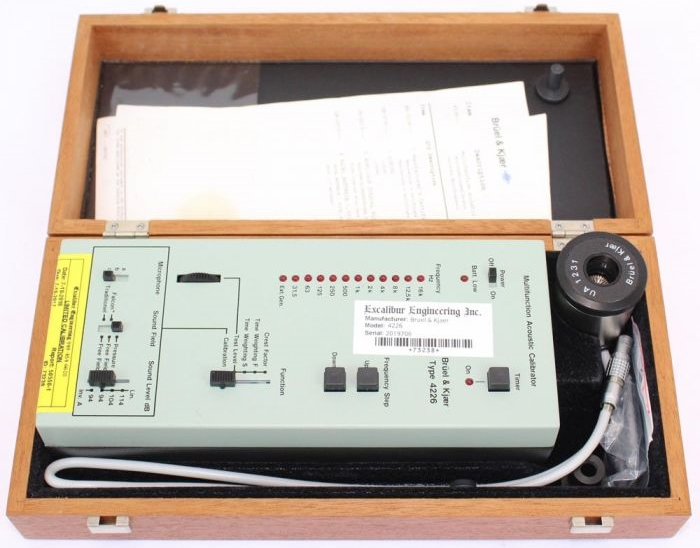
\includegraphics[width=0.35\textwidth]{2_Metodología/Figs/bruel4226}
    \caption*{\footnotesize Tomado de \scriptsize
    \url{https://www.transcat.com/bruel-kjaer-4226-acoustic-calibrator-94-104-and-114db-used}}
\end{figure}

Normalmente, la señal senoidal es generada por algún transductor, como un altavoz o, en el caso de los pistófonos, un pistón mecánico cuyo movimiento genera en la cavidad una velocidad de volumen conocida.
Como ejemplo, en la figura~\ref{fig:bruel_4226} se muestra un calibrador acústico multifunción usado como referencia en muchos laboratorios: el Brüel \& Kjær 4226, que es capaz de generar $\qtylist{94; 104; 114}{\dB}$ en las frecuencias de octava desde $\qty{31.5}{\Hz}$ hasta $\qty{16}{\kHz}$, más la frecuencia de $\qty{12.5}{\Hz}$.

\begin{figure}[!h]
    \caption{Calibrador acústico Brüel \& Kjær 4231 acoplado al micrófono de un sonómetro Brüel \& Kjær 2250.}
    \label{fig:bruel_4231_coupled}
    \centering
    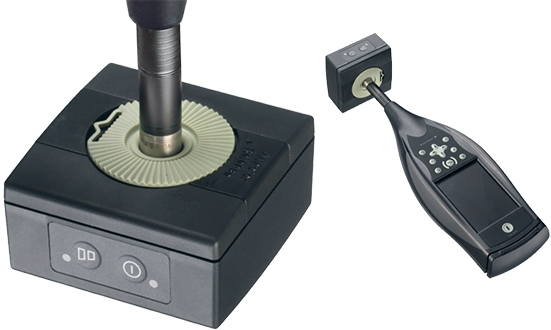
\includegraphics[width=0.45\textwidth]{2_Metodología/Figs/bruel4231coupled}
    \caption*{\footnotesize Tomado de \scriptsize \url{https://www.bksv.com/en/knowledge/blog/sound/getting-started-sound-level-meter}}
\end{figure}
%
Generalmente los calibradores acústicos son empleados para determinar la sensibilidad en campo de presión (típicamente en $\nicefrac{\unit{\mV}}{\unit{\Pa}}$ o en $\unit{\decibel}$ referenciados a $\qty{1}{\V}$) de modelos especificados de micrófonos en configuraciones dadas, pero también es utilizado para verificar o ajustar la sensibilidad de algún dispositivo o sistema de medición acústica.
Un ejemplo de calibrador acoplado para comprobar la indicación de un sonómetro se muestra en la figura~\ref{fig:bruel_4231_coupled}.

La norma \mbox{IEC 60942}~\citeyearpar{IEC_TC29_2017} establece una clasificación de los calibradores según sus especificaciones (límites de aceptación), de la más a la menos restrictiva: Clase LS (\emph{laboratory standard}), clase 1 o clase 2.
La comprobación de que cierto modelo de calibrador cumple con todas las especificaciones normalizadas según su clase la realiza una organización independiente acreditada para hacer pruebas de aprobación de modelo de acuerdo con los lineamientos de la \mbox{IEC 60942} (\mbox{Anexo A}~\citeyear{IEC_TC29_2017}).
Adicionalmente, un usuario de un calibrador acústico debería calibrar periódicamente su instrumento para garantizar la trazabilidad a los estándares nacionales y la confiabilidad de sus resultados.
Esta calibración periódica es llevada a cabo por organismos evaluadores de la conformidad acreditados en \mbox{ISO 17025}~\citeyearpar{ISO_CASCO_2017} para realizar los ensayos periódicos de acuerdo con la \mbox{IEC 60942} (\mbox{Anexo B}~\citeyear{IEC_TC29_2017}).
\vfill

\begin{figure}[!hp]
    \caption{Configuraciones de \emph{hardware} del sonómetro Brüel \& Kjær 2250.}
    \label{fig:bruel_2250_set}
    \centering
    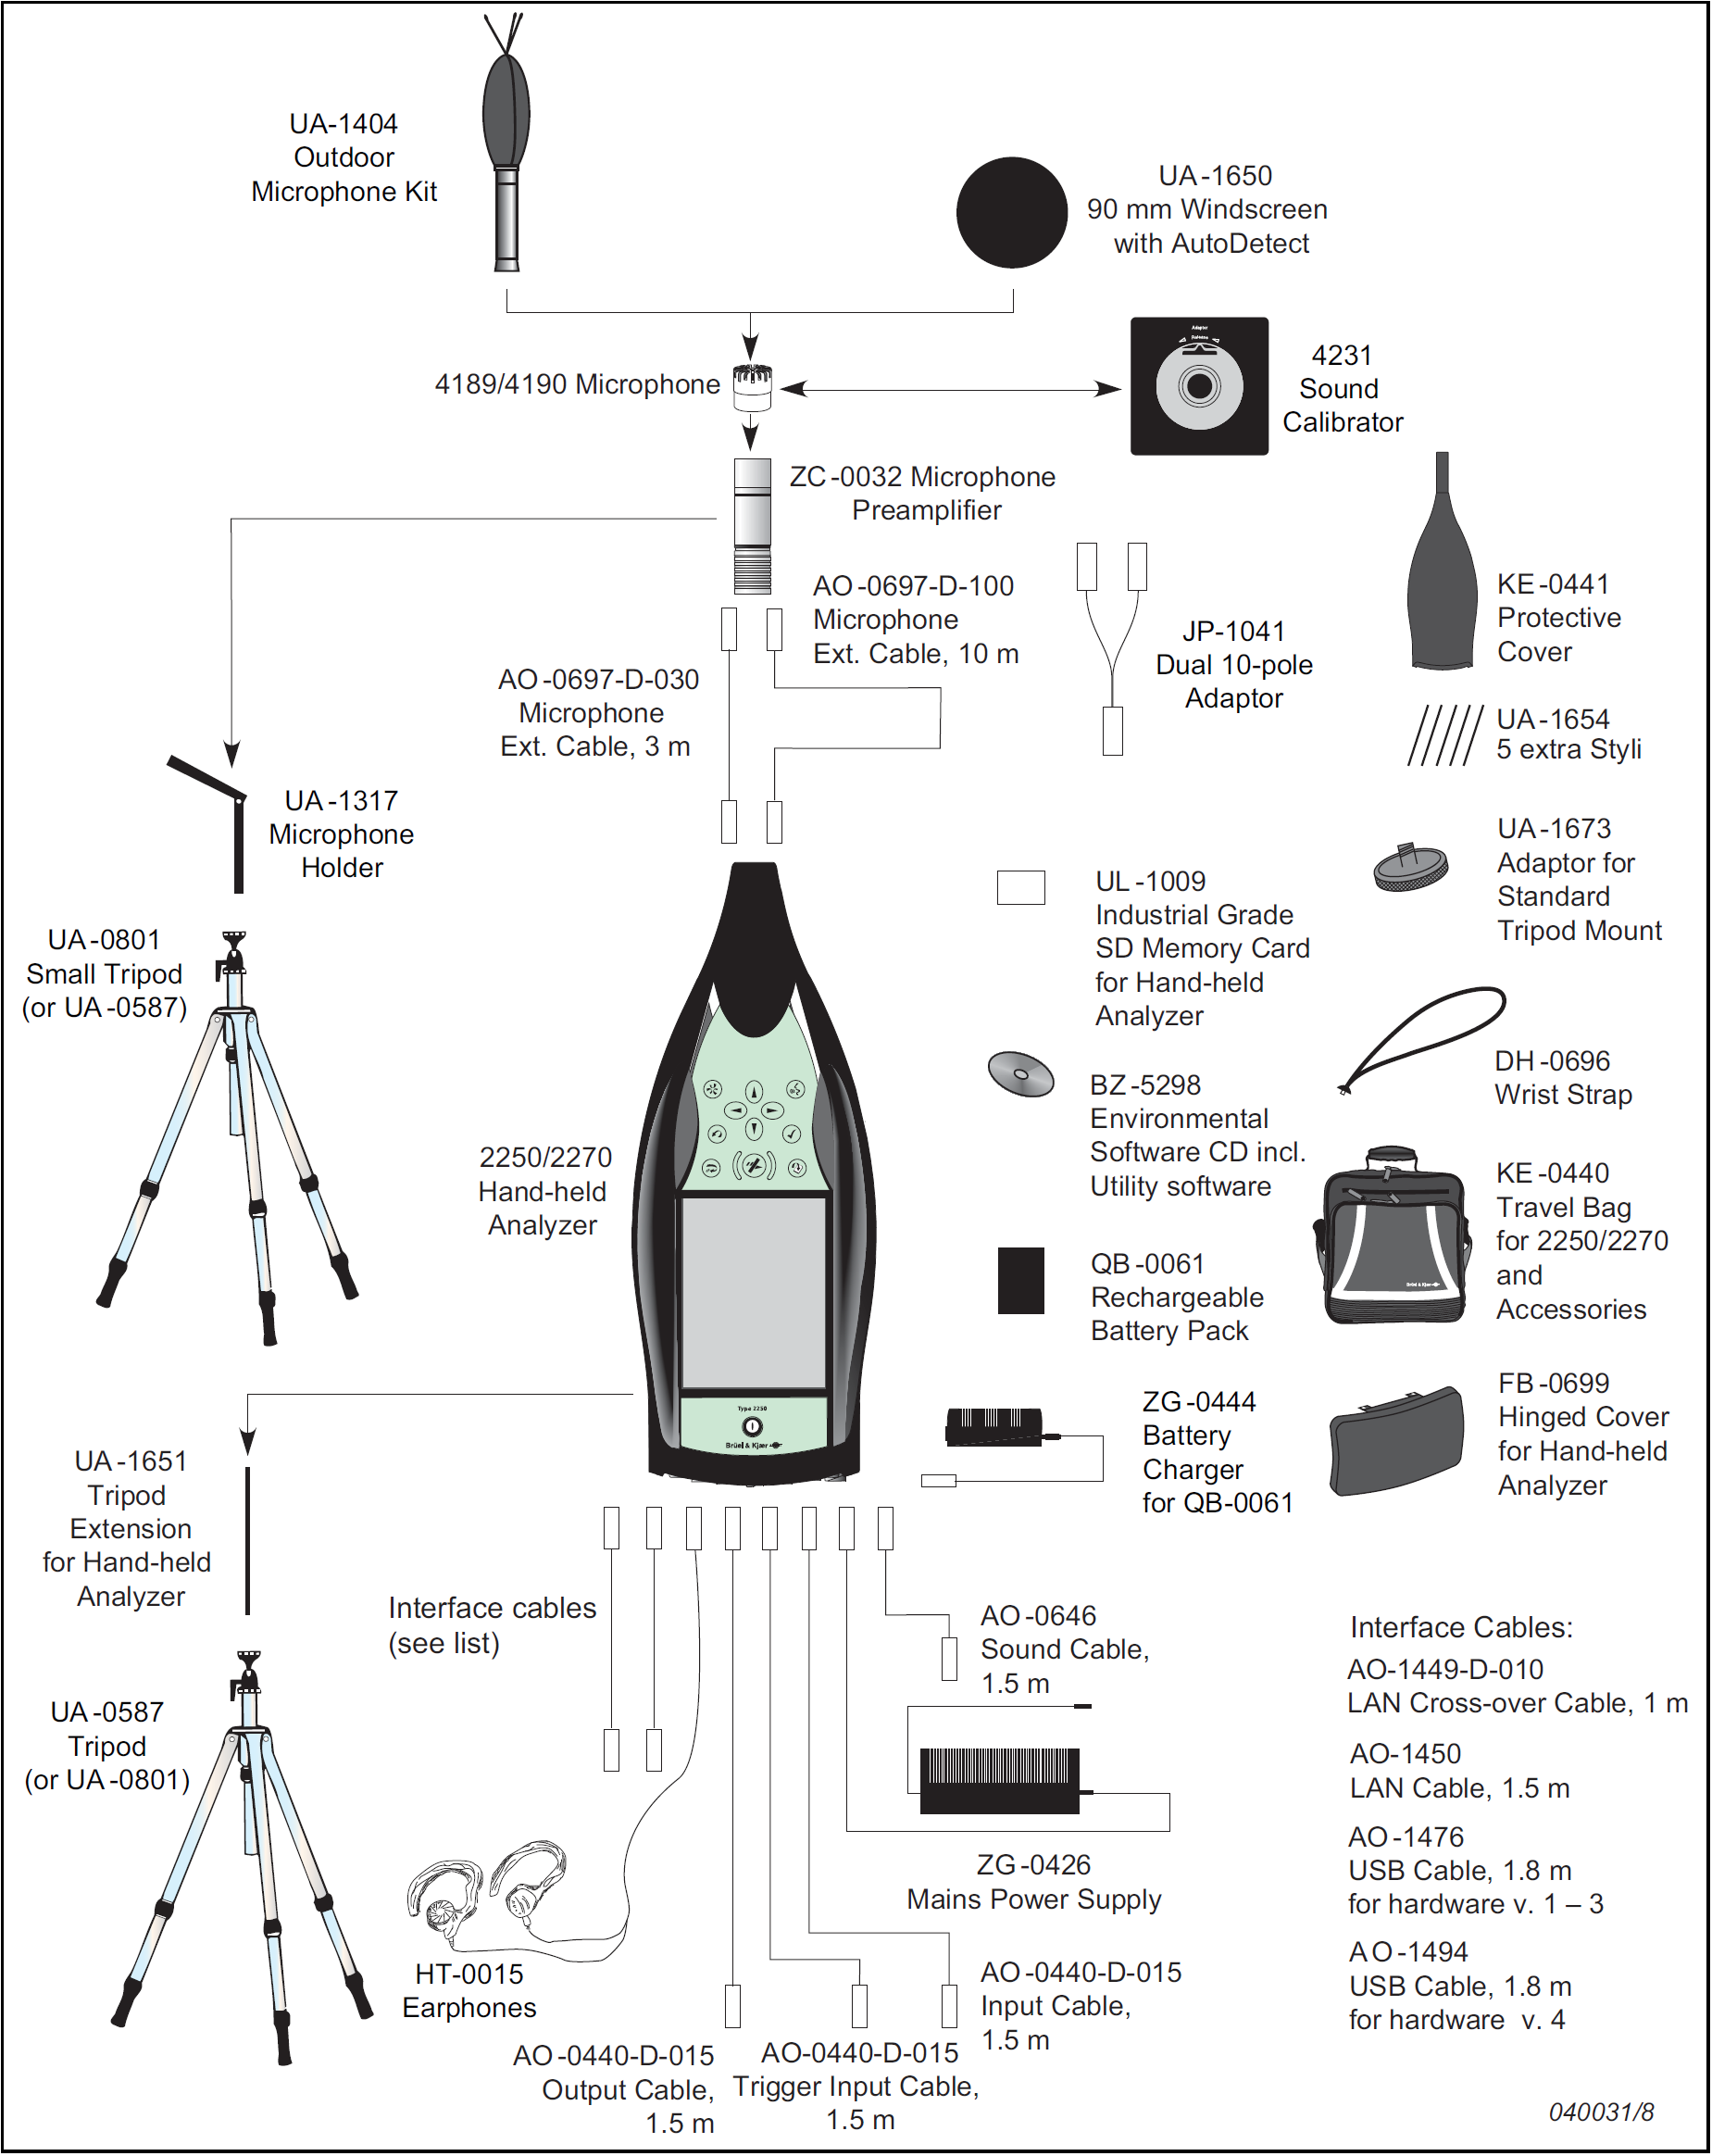
\includegraphics[width=\textwidth]{2_Metodología/Figs/bruel2250set}
    \caption*{\footnotesize Tomado del Manual de Instrucciones \citepalias{Bruel2016}}
\end{figure}

\subsection{Sonómetros integradores}
Brüel \& Kjær, uno de los fabricantes más prominentes de sonómetros define consistentemente los conceptos básicos sobre dichos instrumentos en uno de sus artículos \citepalias{Bruel2021}.
Básicamente, un sonómetro es un instrumento diseñado para medir niveles de sonido de una forma estandarizada;
su respuesta al sonido se asemeja a la del oído humano y proporciona medidas de niveles de presión sonora objetivas y reproducibles.
Generalmente, los sonómetros son empleados en el monitoreo de ruido proveniente de diversas fuentes sonoras, como plantas industriales, tráfico rodado, aeronáutico o ferroviario, conciertos, etc.
Como se puede ver en la figura~\ref{fig:bruel_2250_set}, un sonómetro típico consta de un micrófono, un preamplificador, una unidad de procesamiento de señal (interna) y una pantalla.
Regularmente el preamplificador hace parte del cuerpo del sonómetro, pero no siempre es el caso;
un sonómetro podría estar provisto de cables de extensión que separen el preamplificador de la unidad de procesamiento.

En cuanto al flujo de señal, el micrófono es un transductor electroacústico que transforma la señal acústica en una señal eléctrica.
La mayoría de los micrófonos empleados en mediciones acústicas son de condensador, y gracias a su construcción es el mejor tipo para garantizar precisión, estabilidad y confiabilidad en los resultados.\ No obstante, la señal eléctrica proporcionada por un micrófono es de baja amplitud (aún con micrófonos de alta gama cuya sensibilidad se encuentra típicamente en el orden de los $50\,\nicefrac{\unit{\mV}}{\unit{\Pa}}$, por lo que se requiere una amplificación para que la unidad de procesamiento manipule la señal en un nivel adecuado, este es el objetivo del preamplificador.
Luego, en la unidad de procesamiento se ejecutan diferentes cálculos a partir de la señal.
Los mínimos requeridos por la norma internacional \mbox{IEC 61672--1}~\citeyearpar{IEC_TC29_2013_1} y utilizados en este proyecto se detallan a continuación.

\begin{figure}[!h]
    \caption{Gráfico de las ponderaciones frecuenciales $A$, $C$ y $Z$.}
    \label{fig:frequency_weightings}
    \centering
    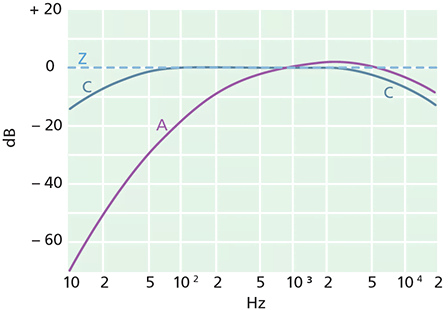
\includegraphics[width=0.54\textwidth]{2_Metodología/Figs/frequency-weighings}
    \caption*{\footnotesize Tomado de \citepalias{Bruel2021}.}
\end{figure}
%
\textbf{Ponderación frecuencial:} Diferencia (como una función especificada de la frecuencia) entre el nivel de la señal ponderada en frecuencia indicado en el dispositivo de presentación de resultados y el nivel correspondiente de una señal de entrada sinusoidal de amplitud constante \citepalias{IEC_TC29_2013_1}.
En la figura~\ref{fig:frequency_weightings} se pueden ver gráficamente las ponderaciones frecuenciales.

Estas ponderaciones frecuenciales estandarizadas $A$, $C$, o $Z$, para las bandas de tercio de octavas están definidas en la \mbox{IEC61672--11} (\mbox{Tabla }~\citeyear{IEC_TC29_2013_1}).
En concreto, cada una de estas ponderaciones modifican la respuesta del sonómetro frente a diferentes frecuencias de sonido.
Por ejemplo, la ponderación $A$ asemeja la respuesta en frecuencia al comportamiento del oído humano en en un rango medio de niveles, tomando como referencia la curva de igual sonoridad de $\qty{40}{\dB}$~\citep{Fletcher1933}, por tal motivo es el más empleado en ruido ambiental y ocupacional.
Pero el oído humano no tiene un comportamiento lineal, y la percepción del sonido varía con el nivel.
La ponderación $C$ está basada en la curva de igual sonoridad de $\qty{100}{\dB}$, por eso esta es empleada en la evaluación de niveles pico de sonidos altos.
Finalmente, la ponderación \emph{zero} $(Z)$ es completamente plana en todo el rango de frecuencias (sin tener en cuenta la respuesta del micrófono).

\textbf{Ponderación temporal:} Es una función exponencial temporal que modifica la respuesta temporal del sonómetro frente a las variaciones en el nivel de presión sonora.
Una comparación entre las respuestas en el tiempo de cada ponderación temporal se muestra en la siguiente figura.
%
\begin{figure}[!h]
    \caption{Gráfico de las respuestas en el tiempo de las ponderaciones temporales \emph{fast}, \emph{slow} e \emph{impulse}.}
    \label{fig:time_weightings}
    \centering
    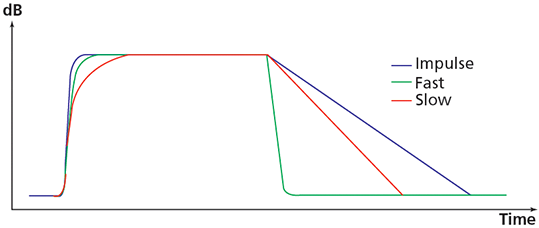
\includegraphics[width=0.55\textwidth]{2_Metodología/Figs/time-weightings}
    \caption*{\footnotesize Tomado de \citepalias{Bruel2021}.}
\end{figure}

Esta función exponencial obedece a una constante de tiempo especificada que depende de la ponderación temporal elegida, bien sea F (\emph{fast}, $\tau_F = \qty{125}{\ms}$), S (\emph{slow}, $\tau_S = \qty{1}{\s}$) o I (\emph{impulse}, $\tau_I = \qty{35}{\ms}$).
Por lo tanto, tal como lo define la norma, para una señal con ponderación $X$, el nivel de sonido con ponderación temporal $Y$ está dado por la siguiente ecuación:
%
\begin{equation}
    \label{eq:time_weighted_level}
    L_{XY}(t) = 10 \log\left(\frac{\frac{1}{\tau_Y}\,
    \int_{-\infty}^t p_X^2\left(\xi\right)\,e^{\nicefrac{-\left(t - \xi\right)}{\tau_Y}}\,\mathrm{d}\xi}
    {p_0^2}\right) \unit{\dB}.
\end{equation}
%
Donde $\tau_Y$ es la constante de tiempo en segundos de la ponderación temporal, $\xi$ es una variable ficticia del tiempo de integración desde un instante de tiempo en el pasado $(-\infty)$ hasta el instante de observación $t$, $p_X\left(\xi\right)$ es la señal de presión acústica instantánea con ponderación frecuencial $X$, y $p_0$ es el valor de referencia de $\qty{20}{\micro\Pa}$.

Consecuentemente, un nivel de sonido, objeto de evaluación en las pruebas aquí implementadas puede ser $L_{AF}$, $L_{AS}$, $L_{CF}$, $L_{CS}$, $L_{ZF}$ o $L_{ZS}$ para las ponderaciones frecuenciales $A$, $C$, o $Z$ y para las ponderaciones temporales \emph{fast} o \emph{slow}.
El resultado de la medición de nivel de sonido es mostrado directamente en la pantalla del sonómetro o alguna otra herramienta de visualización como una interfaz web.
En algunos sonómetros según su tecnología y disposiciones del fabricante, el resultado de medición es enviado vía serial o en forma de una señal DC o AC de amplitud proporcional al nivel de sonido.

La norma \mbox{IEC 61672--1}~\citeyearpar{IEC_TC29_2013_1} establece una clasificación de los sonómetros según sus especificaciones: clase 1 o clase 2.
La comprobación de que cierto modelo de sonómetro cumple con todas las especificaciones normalizadas, según su clase, la realiza una organización independiente acreditada para hacer pruebas de aprobación de modelo de acuerdo con los lineamientos de la \mbox{IEC61672--22}~\citeyearpar{IEC_TC29_2013_2}.
Pero también un usuario de un sonómetro debería calibrar periódicamente su instrumento para garantizar la trazabilidad a los estándares nacionales y la confiabilidad de sus resultados.
Esta calibración periódica es llevada a cabo por organismos evaluadores de la conformidad acreditados en \mbox{ISO 17025}~\citeyearpar{ISO_CASCO_2017} para realizar los ensayos periódicos de acuerdo con la \mbox{IE61672--3-3}~\citeyearpar{IEC_TC29_2013_3}.

Adicionalmente, la sensibilidad del transductor (micrófono) y la respuesta de los circuitos electrónicos puede variar con el paso del tiempo presentando unas pequeñas derivas o también pueden verse afectadas por las condiciones ambientales como la temperatura y la humedad.
Por esto, es una buena práctica verificar regularmente la sensibilidad del sonómetro (preferiblemente antes y después de cada campaña de medición).
De este modo, el sonómetro será ajustado a un nivel de referencia conocido emitido por un calibrador acústico cuyo nivel tenga trazabilidad metrológica.


\section{Métodos normalizados}

Las especificaciones y metodología de calibración de instrumentación acústica y de vibraciones son normalizadas por el comité técnico 29 de la Comisión Electrotécnica Internacional (IEC) en colaboración con la Organización Internacional de Metrología Legal (OIML).
A continuación, un resumen del proceso de calibración de calibradores acústicos y sonómetros, con especial enfoque en los pasos operativos, más que en las disposiciones preliminares de las normas.

\subsection{Descripción general de la calibración periódica de calibradores acústicos de acuerdo con la \mbox{IEC 60942:2017}}
\label{subsec:acoustic_calibrators_calibration_description}

En la siguiente figura se presenta un diagrama que describe en general el proceso de calibración de calibradores acústicos, el cual es explicado en detalle a continuación.
%
\begin{figure}[h]
    \caption{Diagrama de flujo general de la calibración periódica de calibradores acústicos.}
    \label{fig:acoustic_calibrator_calibration_flowchart}
    \centering
    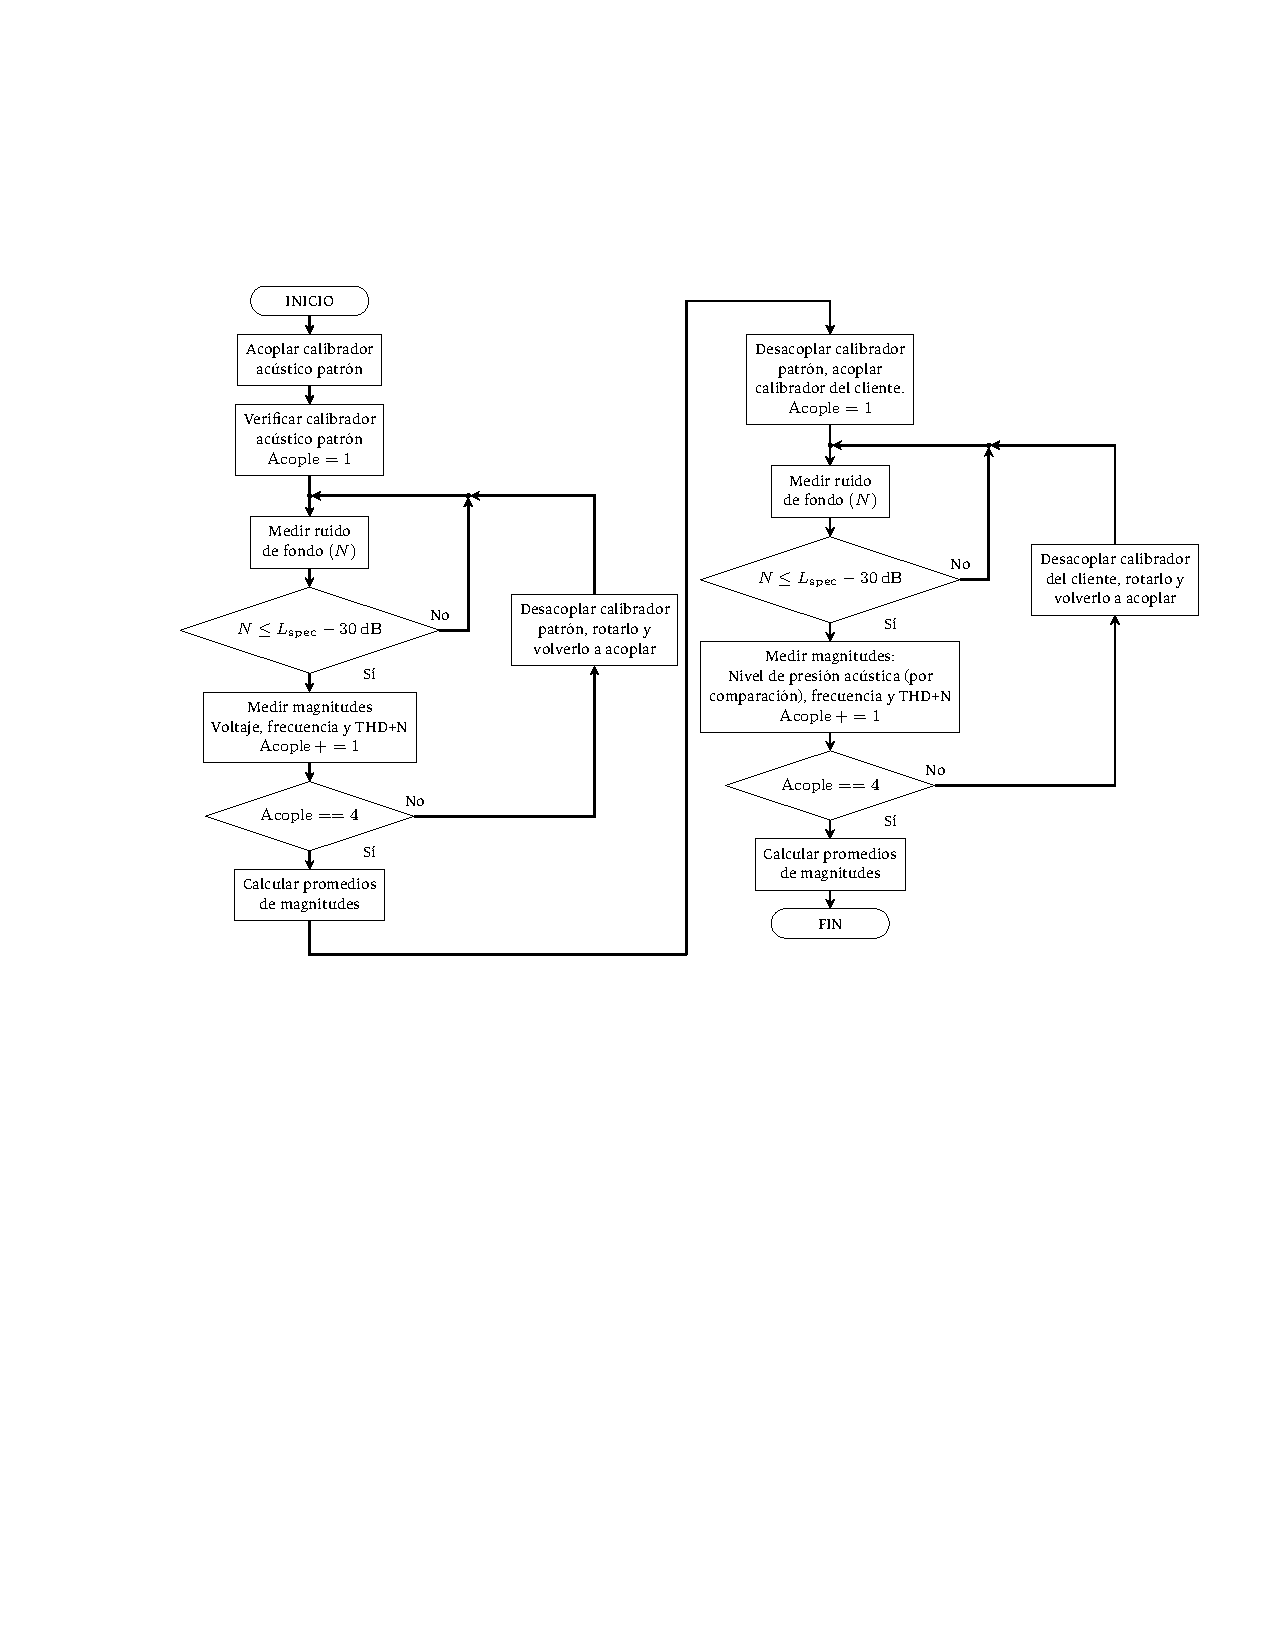
\includegraphics[width=\textwidth]{2_Metodología/IEC60942Flowchart}
    \caption*{\footnotesize Fuente: Elaboración propia.}
\end{figure}

Tal como se describe en la \mbox{IEC 60942} (\mbox{Anexo B}~\citeyear{IEC_TC29_2017}), el calibrador acústico o pistófono con todos sus accesorios necesarios (como adoptadores o barómetro) debe ser entregado junto con el manual de instrucciones, si este es requerido por el laboratorio de calibración.
Luego, se hace una inspección visual del calibrador acústico, verificando que todos los controles están funcionando y que la fuente de alimentación está operando dentro de los límites especificados en el manual de instrucciones.
En seguida, se toman en cuenta o se realizan las siguientes secciones.

\textbf{Orientación para los ensayos}.
Si en el manual de instrucciones se especifica alguna orientación del calibrador acústico, esta debe ser la utilizada en la calibración periódica.

\textbf{Ruido ambiental}.
Para evitar que el ruido ambiental afecte las mediciones, las pruebas sólo se realizan si el nivel de presión sonora con el calibrador acoplado al micrófono (pero con el calibrador apagado) es por lo menos $\qty{30}{\dB}$ por debajo del nivel especificado que se está midiendo.

\textbf{Influencia de las condiciones ambientales}.
Cuando es apropiado, la información suministrada en el manual de instrucciones sobre la influencia de la presión estática debe ser aplicada para corregir el nivel de presión medido a la presión estática de referencia.

\textbf{Nivel de presión sonora}.
Después de acoplar el calibrador acústico al micrófono, se debe dejar el tiempo de estabilización indicado en el manual de instrucciones.
Luego, el nivel de presión sonora generado por el calibrador debe ser medido como un promedio de los valores instantáneos obtenidos durante un periodo $t_{\mathrm{op}}$ de entre $\qtylist{20;25}{\s}$ de operación.

Para medir el nivel de presión sonora hay propuestos dos métodos en la norma internacional: Usando un micrófono de referencia o usando un calibrador acústico de referencia para comparación.
En este proyecto se utiliza el segundo, en el que el nivel del calibrador bajo prueba es determinado por comparación contra el nivel generado por un calibrador acústico calibrado cuya trazabilidad metrológica esté establecida.
Como la señal a analizar es eléctrica, el nivel de presión se determina como una diferencia logarítmica:
\begin{equation}
    \label{eq:spl_from_voltage}
    L = L_{\mathrm{ref}} + 20\,\log\left(\frac{\bar{v}}{\bar{v}_{\mathrm{ref}}}\right).
\end{equation}
%
En que $L$ es el nivel de presión sonora del calibrador acústico bajo calibración, $L_{\mathrm{ref}}$ es el nivel de presión certificado del calibrador acústico patrón, y $\bar{v}$ y $\bar{v}_{\mathrm{ref}}$ son el voltaje medio medido con el calibrador del cliente y con el calibrador de referencia durante el tiempo $t_{\mathrm{op}}$ respectivamente.

El nivel de presión sonora debe ser medido al menos tres veces, cada vez acoplando el micrófono y el calibrador acústico antes de la medición y desacoplándolo después.
En cada nuevo acoplamiento se debe rotar el micrófono sobre su eje.
La diferencia absoluta entre el nivel medido medio y el nivel especificado no debe exceder los límites establecidos en la \mbox{IEC 60942} (\mbox{Tabla 2}~\citeyear{IEC_TC29_2017}), según la clase del calibrador y la frecuencia medida.
La medición de nivel de presión sonora debe ser repetida para cada combinación de nivel y frecuencia que indique el manual de instrucciones que cumple con las especificaciones de la norma.

\textbf{Frecuencia}, debe ser medida con el calibrador acoplado al micrófono como un promedio de los valores instantáneos obtenidos durante el tiempo $t_{\mathrm{op}}$, para cada frecuencia disponible en el calibrador, de la cual se indique en el manual que cumple con las especificaciones de la norma.
El valor absoluto de la diferencia porcentual a cada frecuencia medida (ver ecuación~\ref{eq:porcentual_difference}) y la correspondiente frecuencia especificada no debe exceder los límites establecidos en la \mbox{IEC 60942} (\mbox{Tabla 4}~\citeyear{IEC_TC29_2017}), según la clase del calibrador.
%
\begin{equation}
    \label{eq:porcentual_difference}
    \%error = \left|\frac{\bar{f}}{f_{\mathrm{spec}}} - 1\right| \times 100.
\end{equation}
%
En que $\bar{f}$ es la frecuencia media medida durante el tiempo $t_{\mathrm{op}}$ y $f_{\mathrm{spec}}$ es la frecuencia especificada bajo calibración.

\textbf{Distorsión armónica total más ruido (THD+N)}, la distorsión de la señal generada por el calibrador debe medirse con un ancho de banda de $\qty{22.4}{\Hz}$ a $\qty{22.4}{\kHz}$, como un promedio de los valores instantáneos obtenidos durante el tiempo $t_{\mathrm{op}}$, en los niveles máximo y mínimos disponibles a cada frecuencia de los que se indique en el manual que cumple con las especificaciones de la norma.
La THD+N puede ser medida utilizando un filtro de rechazo (medidor de factor de distorsión) o un analizador FFT. La THD+N medida no debe exceder los límites establecidos en la \mbox{IEC 60942} (\mbox{Tabla 7}~\citeyear{IEC_TC29_2017}), según la clase del calibrador.
Es obligatorio que la magnitud medida sea no sólo distorsión armónica total, sino distorsión armónica total \emph{más} ruido, reportada en porcentaje ($\%$).

\subsection{Descripción general de las pruebas periódicas seleccionadas de acuerdo con la \mbox{IEC 61672-3:2013}}
\label{subsec:slm_calibration_description}

\tikzmath{\x1 =1; \x2 = 3/5; \x3 = 3.1/6;}
\definecolor{block_blue}{HTML}{d4e1f5}
\begin{figure}[h]
    \caption{Diagrama de bloques del proceso de medición en la calibración periódica de sonómetros de acuerdo con la \mbox{IEC 61672-3:2013}.}
    \label{fig:slm_calibration_flowchart}
    \centering
    \begin{tikzpicture}[font=\scriptsize, minimum width=1cm, minimum height=1.5cm, align=center]
        \node (process1) at (-10, 0) [draw, process]{Recepción de \\ items de \\ calibración};
        \node (process2) [draw, process, right=\x1cm of process1]{Inspección \\ visual};
        \node (process3) [draw, process, right=\x1cm of process2,
            fill=block_blue]{Verificación \\ del calibrador \\ acústico};
        \node (process4) [draw, process, right=\x1cm of process3, fill=block_blue]{Verificación \\ de fuente de \\ alimentación};
        \node (process5) [draw, process, right=\x1cm of process4]{Ruido \\ intrínseco};
        \node (process6) [draw, process, right=\x1cm of process5]{Indicación a la \\ frecuencia de \\ comprobación de \\ la calibración};
        \node (process7) [draw, process, below=0.3cm of process6]{Una ponderación \\ frecuencial con \\ señales acústicas};
        \node (process8) [draw, process, left=\x2cm of process7, fill=block_blue]{Verificación \\ de fuente de \\ alimentación};
        \node (process9) [draw, process, left=\x2cm of process8, fill=block_blue]{Ponderaciones \\ frecuenciales y \\ temporales a $\qty{1}{\kHz}$};
        \node (process10) [draw, process, left=\x2cm of process9, fill=block_blue]{Ponderación \\ frecuencial con \\ señales eléctricas};
        \node (process11) [draw, process, left=\x2cm of process10, fill=block_blue]{Linealidad en el \\ rango de niveles \\ de referencia};
        \node (process12) [draw, process, below=0.3cm of process1]{Respuesta a \\ trenes de \\ onda};
        \node (process13) [draw, process, below=0.3cm of process12]{Nivel de \\ sonido $C$ \\ de pico};
        \node (process14) [draw, process, right=\x3cm of process13]{Indicación \\ de \\ sobrecarga};
        \node (process15) [draw, process, right=\x3cm of process14]{Estabilidad \\ a niveles \\ elevados};
        \node (process16) [draw, process, right=\x3cm of process15]{Estabilidad a \\ largo plazo};
        \node (process17) [draw, process, right=\x3cm of process16, fill=block_blue]{Verificación \\ de fuente de \\ alimentación};
        \node (process18) [draw, process, right=\x3cm of process17, fill=block_blue]{Estimación de \\ incertidumbre de \\ medición};
        \node (process19) [draw, process, below=0.3cm of process7]{Generación de \\ certificado de \\ calibración};

        \draw [arrow] (process1) -- (process2);
        \draw [arrow] (process2) -- (process3);
        \draw [arrow] (process3) -- (process4);
        \draw [arrow] (process4) -- (process5);
        \draw [arrow] (process5) -- (process6);
        \draw [arrow] (process6.east) -- +(0.3cm, 0cm) |- (process7);
        \draw [arrow] (process7) -- (process8);
        \draw [arrow] (process8) -- (process9);
        \draw [arrow] (process9) -- (process10);
        \draw [arrow] (process10) -- (process11);
        \draw [arrow] (process11) -- (process12);
        \draw [arrow] (process12.west) -- +(-0.3cm, 0cm) |- (process13);
        \draw [arrow] (process13) -- (process14);
        \draw [arrow] (process14) -- (process15);
        \draw [arrow] (process15) -- (process16);
        \draw [arrow] (process16) -- (process17);
        \draw [arrow] (process17) -- (process18);
        \draw [arrow] (process18) -- (process19);
    \end{tikzpicture}
    \caption*{\footnotesize Fuente: Elaboración propia.}
\end{figure}
%
En el diagrama de bloques de la figura~\ref{fig:slm_calibration_flowchart} se presenta de forma general el proceso de calibración periódica de sonómetros.
Los bloques resaltados en azul son los procesos objeto de automatización en este proyecto\footnote{Aún con la automatización de estas actividades, hay tareas que deben realizarse manualmente por el usuario dadas las limitaciones físicas o de la naturaleza misma de los equipos. Por ejemplo, el usuario debe ajustar la orientación del calibrador acústico, encenderlo o apagarlo, configurar en el sonómetro los indicadores en pantalla, etc.}.
A continuación se describen en detalle las etapas en el proceso de calibración.

En principio, de conformidad con la \mbox{IEC 661672--3}~\citeyearpar{IEC_TC29_2013_3}, el sonómetro con todos sus accesorios necesarios (como preamplificador, micrófono, cable de extensión o adaptador de impedancia) debe ser entregado junto con el manual de instrucciones, si este es requerido por el laboratorio de calibración.
Toda la información necesaria para los ensayos periódicos debe estar disponible, como correcciones de campo libre, rangos de medición, niveles de referencia, etc.
Se debe contar con un calibrador acústico conforme con las especificaciones de la \mbox{IEC 60942}~\citeyearpar{IEC_TC29_2017} según su clase, ya sea suministrado por el cliente o por el laboratorio.

Luego, se hace una inspección preliminar del sonómetro y todos sus accesorios, verificando que todos los controles están funcionando, que la pantalla está en buen estado, que no haya acumulación de material extraño en la rejilla o membrana del micrófono y que otros elementos esenciales estén en un funcionamiento adecuado.
Después se verifica que la fuente de alimentación está operando dentro de los límites especificados en el manual de instrucciones.
La fuente de alimentación será verificada nuevamente después de los ensayos con señales acústicas y después de los ensayos con señales eléctricas.
A continuación, se detallan las pruebas que serán efectuadas.
Para todas las pruebas eléctricas se emplea el dispositivo de entrada (acoplador de impedancia) recomendado por el fabricante del sonómetro o uno que tenga una capacitancia similar que emule adecuadamente la carga del micrófono en el preamplificador.

\subsubsection{Indicación a la frecuencia de comprobación de la calibración}
El calibrador acústico entregado por el cliente o proporcionado por el laboratorio se acopla al micrófono del sonómetro, y, si es necesario, se ajusta el sonómetro para indicar el nivel de presión acústica requerido en las condiciones ambientales en las que se realizan los ensayos.
Las indicaciones antes y después del ajuste deben registrarse.
Se debe tomar en cuenta el efecto de la presión estática sobre el calibrador acústico empleado.
Este calibrador ya debió haber sido verificado previamente, según el procedimiento descrito en la sección~\ref{subsec:acoustic_calibrators_calibration_description}.

Después de haber ajustado el sonómetro en respuesta al nivel generado por el calibrador, un paso necesario (antes de continuar con las otras pruebas) es determinar el voltaje que produce una indicación del nivel de referencia.
La siguiente ecuación es empleada para determinar ese voltaje:
%
\begin{equation}
    \label{eq:reference_voltage}
    v_{\mathrm{ref}} = 10\,\hat{\mkern6mu}\left(\frac{L_{v,l}+\nicefrac{\left(L_{v,u} - L_{v,l}\right)}{2}}{20}\right).
\end{equation}
%
Donde $v_{\mathrm{ref}}$ es el voltaje medio en una escala logarítmica que produce una indicación del nivel de referencia, $L_{v,l}$ es el nivel de voltaje inferior del intervalo que produce una indicación del nivel de referencia, y $L_{v,u}$ el nivel de voltaje superior.
Los niveles de voltaje son referenciados a $\qty{1}{\V}$.
En concreto, este voltaje de referencia es el voltaje en la mitad (en una escala logarítmica) de un intervalo de voltajes que producen todos una misma indicación del nivel de referencia.
Con el voltaje de referencia se calculan los voltajes correspondientes a los niveles de señal en las demás pruebas.

\subsubsection{Ponderaciones frecuenciales y temporales a 1 kHz}
Se utiliza una señal eléctrica continua de $\qty{1}{\kHz}$ con una amplitud tal que produzca una indicación del nivel de referencia en el sonómetro $\left(\text{i.e. } v_{\mathrm{ref}}\right)$  y se siguen los pasos a continuación:
%
\begin{description}
    \item[PFT-1] Registrar el nivel indicado en las ponderaciones frecuenciales $A$, $C$ y $Z$ (según estén disponibles) con el sonómetro ajustado en ponderación temporal $F$ o nivel promediado en el tiempo\footnote{Como en este trabajo se busca reconocer el resultado instantáneo mostrado en pantalla, el nivel elegido preferiblemente es el que tiene ponderación temporal F.}; i.e. $L_{AF}, L_{CF}, L_{ZF}, L_{Aeq}, L_{Ceq}$ o $L_{Zeq}$.

    \item[PFT-2\label{itm:time_frequency_weight_registration}] Registrar el nivel indicado en las ponderaciones temporales F y S, y el nivel promediado en el tiempo\footnote{El nivel promediado en el tiempo sólo sería posible registrarlo automáticamente si este es mostrado en pantalla.} (según estén disponibles) con el sonómetro ajustado en ponderación frecuencial $A$; i.e. $L_{AF}, L_{AS}$ o $L_{Aeq}$.

    \item[PFT-3] Calcular las desviaciones de los niveles ponderados en frecuencia $C$ y $Z$ respecto al ponderado en frecuencia $A$ del paso 1.
    Estas desviaciones no deben superar los límites de aceptación de $\pm\qty{0.2}{\dB}$.

    \item[PFT-4] Calcular las desviaciones del nivel promediado en el tiempo y del nivel con ponderación temporal S, respecto al nivel con ponderación temporal F del paso~\ref{itm:time_frequency_weight_registration}.
    Estas desviaciones no deben superar los límites de aceptación de $\pm\qty{0.1}{\dB}$.
\end{description}

\subsubsection{Ponderaciones frecuenciales con señales eléctricas}

Se utilizan señales eléctricas sinusoidales continuas para todas las ponderaciones frecuenciales reguladas en la \mbox{IEC 61672--1}~\citeyearpar{IEC_TC29_2013_1} (que estén disponibles en el sonómetro).
Y se siguen los pasos a continuación:
%
\begin{description}
    \item[PFSE-1] Se ajusta el sonómetro para mostrar niveles de sonido con ponderación temporal F, niveles promediados en el tiempo o niveles de exposición sonora \footnote{Como en este trabajo se busca reconocer el resultado instantáneo mostrado en pantalla, el nivel elegido es preferiblemente el que tiene ponderación temporal F.}.

    \item[PFSE-2] Se ajusta el sonómetro en el rango de niveles de referencia y se envía una señal de $\qty{1}{\kHz}$ cuya amplitud produzca una indicación en el sonómetro que sea $\qty{45}{\dB}$ menos que el límite superior indicado en el manual de instrucciones para el rango de funcionamiento lineal a $\qty{1}{\kHz}$.

    Para automatizar este paso, se usa la siguiente ecuación:
%
    \begin{equation}
        \label{eq:voltage_1khz}
        v_{\qty{1}{\kHz}} = 10\,\hat{\mkern6mu}
        \left(\frac{20\,\log\left(v_{\mathrm{ref}}\right) + L_{\mathrm{ref}} - \left(L_{u@\qty{1}{\kHz}} - 45\right)}{20}\right).
    \end{equation}
%
    En que $v_{\qty{1}{\kHz}}$ es el voltaje que produce una indicación de $\qty{45}{\dB}$ menos que el límite superior del rango lineal a $\qty{1}{\kHz}$; $v_{\mathrm{ref}}$ es el voltaje que produce una indicación del nivel de referencia $L_{\mathrm{ref}}$; y, $L_{u@\qty{1}{\kHz}}$ es el límite superior del rango lineal a $\qty{1}{\kHz}$ especificado en el manual de instrucciones.

    \item[PFSE-3] Se registran los niveles de las señales de entrada y las correspondientes indicaciones.
    Para sonómetros clase 1 en las nueve frecuencias nominales en intervalos de octava de $\qty{63}{\Hz}$ a $\qty{16}{\kHz}$.
    Para sonómetros clase 2 en las ocho frecuencias nominales en intervalos de octava de $\qty{63}{\Hz}$ a $\qty{8}{\kHz}$.

    En frecuencias diferentes a $\qty{1}{\kHz}$ el voltaje de la señal de entrada se determina mediante
%
    \begin{equation}
        \label{eq:voltage_by_frequency}
        v_f = 10\,\hat{\mkern6mu}\left(\frac{20\,\log\left(v_{\qty{1}{\kHz}}\right) - W_{X,f}}{20}\right).
    \end{equation}
%
    En que $v_f$ es el voltaje de la señal a la frecuencia $f$, $v_{\qty{1}{\kHz}}$ es el voltaje del paso anterior y $W_{X,f}$ es el factor de la ponderación frecuencial elegida $X$ para la frecuencia $f$.

    \item[PFSE-4] Se calculan las ponderaciones frecuenciales relativas como $L_{f} - L_{\qty{1}{\kHz}}$, i.e.\ el nivel indicado a una frecuencia de ensayo menos el nivel indicado a $\qty{1}{\kHz}$.

    \item[PFSE-5] Aplicar factores de corrección a las ponderaciones frecuenciales relativas del paso anterior que den cuenta de:
%
    \begin{description}
        \item[PFSE-5.1] La desviación de la respuesta en frecuencia en campo libre o para incidencia aleatorio de un micrófono en la dirección de referencia respecto a una respuesta en frecuencia uniforme.
        \item[PFSE-5.2] Los efectos de las reflexiones en la carcasa del sonómetro y de la difracción del sonido alrededor del micrófono y del amplificador.
        \item[PFSE-5.3] Si aplica, la influencia de la pantalla antiviento y de cualquier accesorio que sea parte de la configuración normal del sonómetro.
    \end{description}

    \item[PFSE-6] Las ponderaciones frecuenciales relativas corregidas son las desviaciones respecto a los objetivos de diseño según la ponderación frecuencial bajo calibración y no deben exceder los límites de aceptación dados en la \mbox{IEC 61672--1} (\mbox{Tabla 3}~\citeyear{IEC_TC29_2013_1}).
\end{description}

\subsubsection{Linealidad de nivel en el rango de niveles de referencia}
Se utilizan señales eléctricas sinusoidales continuas a una frecuencia de $\qty{8}{\kHz}$ con el sonómetro ajustado en el rango de niveles de referencia, en ponderación frecuencial $A$, y con ponderación temporal F o un nivel promediado en el tiempo, i.e. $L_{AF}$ o $L_{Aeq}$, y se siguen los pasos a continuación:
%
\begin{description}
    \item[LNRR-1] Comenzar con una señal de entrada cuya amplitud produce el punto de partida para los ensayos de linealidad a $\qty{8}{\kHz}$ especificado en el manual de instrucciones.
    Y registrar el nivel indicado.

    \item[LNRR-2] Aumentar el nivel de la señal de entrada en saltos de $\qty{5}{\dB}$ desde el punto de partida hasta un nivel que se encuentre dentro de $\qty{5}{\dB}$ por debajo del límite superior del rango de funcionamiento lineal a $\qty{8}{\kHz}$ especificado en el manual.
    Luego, aumentar en saltos de $\qty{1}{\dB}$ hasta, pero sin incluir, la primera indicación de sobrecarga.
    Se deben registrar las indicaciones del sonómetro en cada punto.

    \item[LNRR-3] Disminuir el nivel de la señal de entrada en saltos de $\qty{5}{\dB}$ desde el punto de partida hasta un nivel que se encuentre dentro de $\qty{5}{\dB}$ por encima del límite inferior del rango de funcionamiento lineal a $\qty{8}{\kHz}$ especificado en el manual.
    Luego, disminuir en saltos de $\qty{1}{\dB}$ hasta, pero sin incluir, la primera indicación de ``por debajo del rango".
    Se deben registrar las indicaciones del sonómetro en cada punto.

    \item[LNRR-4] Calcular las desviaciones de nivel como la diferencia entre el nivel indicado y el nivel previsto.
    Estas desviaciones no deben superar los límites de $\pm\qty{0.8}{\dB}$ para la clase 1 o de $\pm\qty{1.1}{\dB}$ para la clase 2.
\end{description}

Para automatizar esta prueba, el voltaje en el punto de partida se determina como
%
\begin{equation}
    \label{eq:voltaje_start_point}
    v_{L_{\mathrm{start}}} = 10\,\hat{\mkern6mu}
    \left(\frac{20\,\log\left(v_{\mathrm{ref}}\right) +
    L_{\mathrm{start}} - L_{\mathrm{ref}} -
    W_{A,\qty{8}{\kHz}} - E_{A,\qty{8}{\kHz}}}{20}\right).
\end{equation}
%
En que $v_{L_{\mathrm{start}}}$ es el voltaje que causa una indicación del nivel en el punto de partida $L_{\mathrm{start}}$; $v_{\mathrm{ref}}$ es el voltaje que produce una indicación del nivel de referencia, $W_{A,\qty{8}{\kHz}}$ es el factor estandarizado de la ponderación $A$ en la frecuencia de $\qty{8}{\kHz}$ que tiene el valor de $\qty{-1.1}{\dB}$ y $E_{A,\qty{8}{\kHz}}$ es la ponderación relativa a $\qty{1}{\kHz}$ (sin corregir), obtenida en la prueba de ponderaciones frecuenciales en la frecuencia de $\qty{8}{\kHz}$ en la ponderación frecuencial $A$.%, y $R_{\mathrm{FF},\qty{8}{\kHz}}$ es la corrección de campo libre para la frecuencia de $\qty{8}{\kHz}$.

Luego, a partir de ese voltaje en el punto de partida, el voltaje $v_{L_{\mathrm{prev}}}$ para cada punto de calibración o nivel previsto $L_{\mathrm{prev}}$ a lo largo del rango de niveles, se calcula como:
%
\begin{equation}
    \label{eq:voltage_linearity}
    v_{L_{\mathrm{prev}}} = 10\,\hat{\mkern6mu}
    \left(\frac{20\,\log\left(v_{L_{\mathrm{start}}}\right) + L_{\mathrm{prev}} - L_{\mathrm{start}}}{20}\right).
\end{equation}


\section{Instrumentación}\label{sec:instrumentacion}

Los instrumentos presentados a continuación fueron elegidos teniendo en cuenta los requisitos metrológicos para obtener resultados confiables y trazables, como también asegurando que tengan las prestaciones mínimas para implementar el control remoto desde un ordenador.

\begin{figure}[!h]
    \caption{Esquema de conexiones de los instrumentos para la calibración periódica de calibradores acústicos.}
    \label{fig:IEC60942_connections}
    \begin{subfigure}[t]{0.59\textwidth}
        \centering
        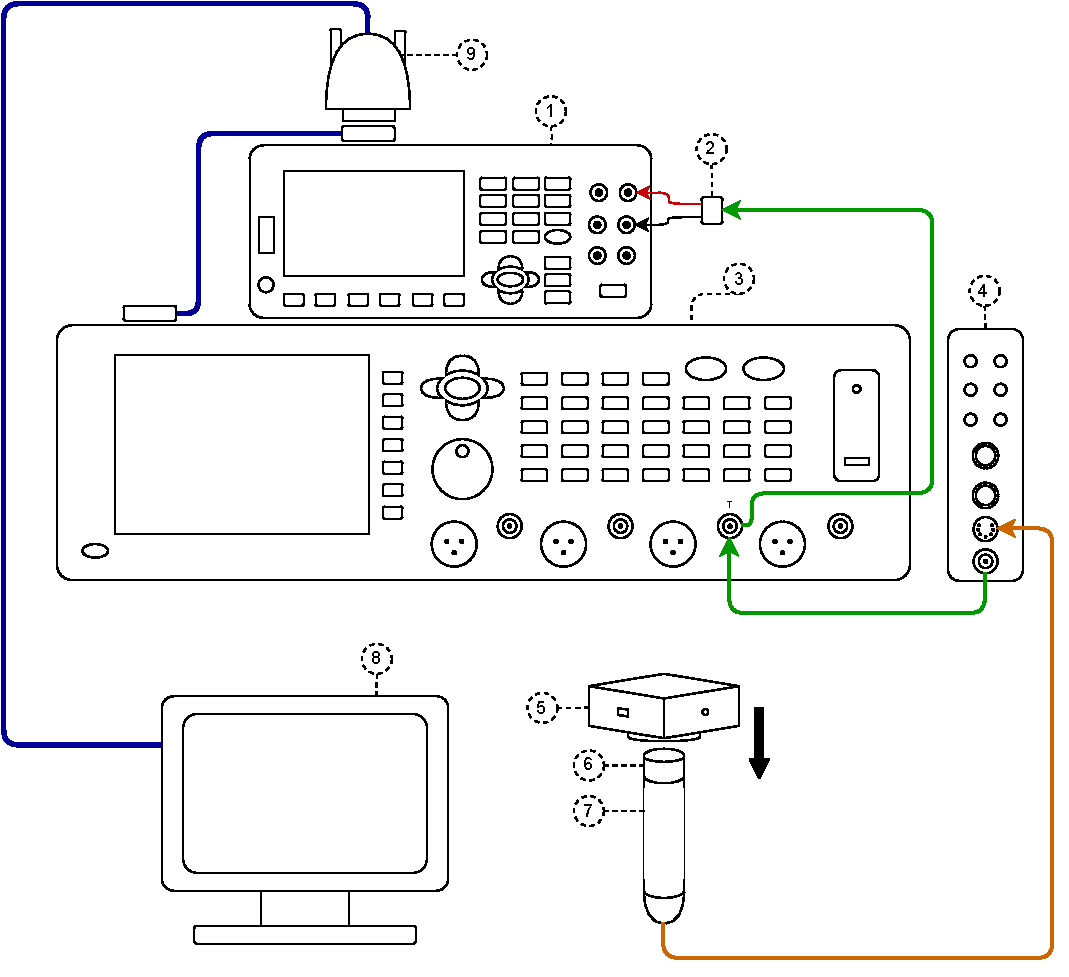
\includegraphics[width=0.95\textwidth]{2_Metodología/Figs/IEC60942connections}
    \end{subfigure}
    \hfill
    \begin{subfigure}[t]{0.4\textwidth}
        \centering
        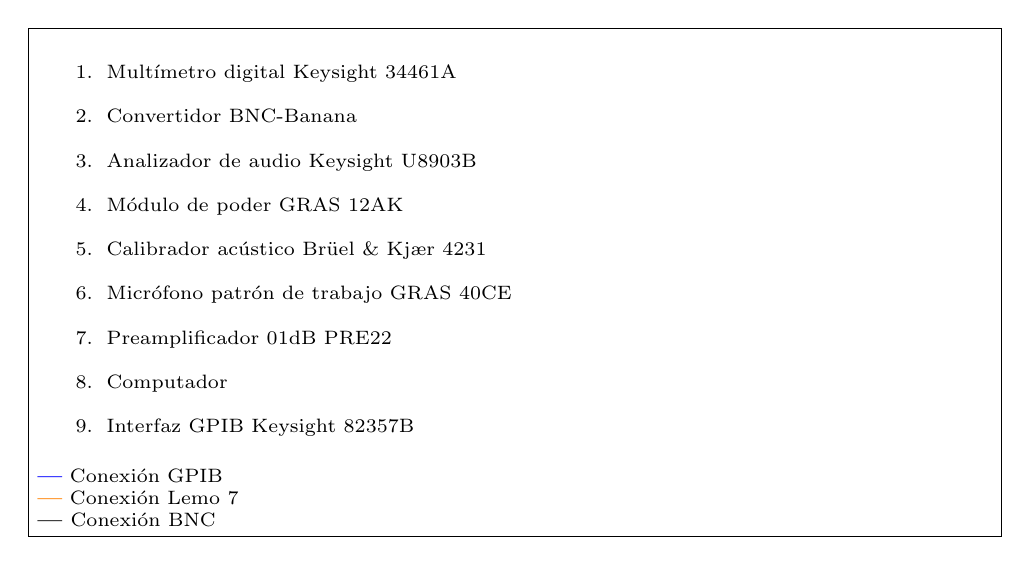
\begin{tikzpicture}
            \node [draw]{\vbox{\scriptsize{
                \begin{enumerate}
                    \item Multímetro digital Keysight 34461A
                    \item Convertidor BNC-Banana
                    \item Analizador de audio Keysight U8903B
                    \item Módulo de poder GRAS 12AK
                    \item Calibrador acústico Brüel \& Kjær 4231
                    \item Micrófono patrón de trabajo GRAS 40CE
                    \item Preamplificador 01dB PRE22
                    \item Computador
                    \item Interfaz GPIB Keysight 82357B
                \end{enumerate}}
            \textbf{\color{blue} —} Conexión GPIB \\
            \textbf{\color{orange} —} Conexión Lemo 7 \\
            \textbf{—} Conexión BNC}};
        \end{tikzpicture}
    \end{subfigure}
    \caption*{\footnotesize Fuente: Elaboración propia.}
\end{figure}

\subsection{Patrones e instrumentos para la calibración periódica de calibradores acústicos}

La interconexión propuesta de los instrumentos empleados en la calibración de calibradores acústicos se presenta en la figura~\ref{fig:IEC60942_connections}.
A continuación se describen las características de cada instrumento.

\begin{figure}[!h]
    \caption{Patrones acústicos para la calibración de calibradores acústicos.}
    \centering
    \begin{subfigure}[t]{0.49\textwidth}
        \centering
        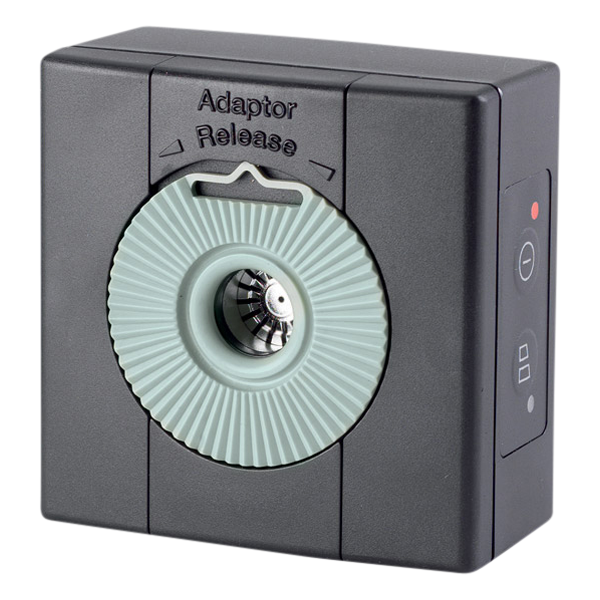
\includegraphics[height=4cm]{2_Metodología/Figs/bruel4231}
        \caption{Calibrador acústico Brüel \& Kjær 4231 usado como patrón de laboratorio.}
        \label{fig:bruel_4231}
    \end{subfigure}
    \hfill
    \begin{subfigure}[t]{0.49\textwidth}
        \centering
        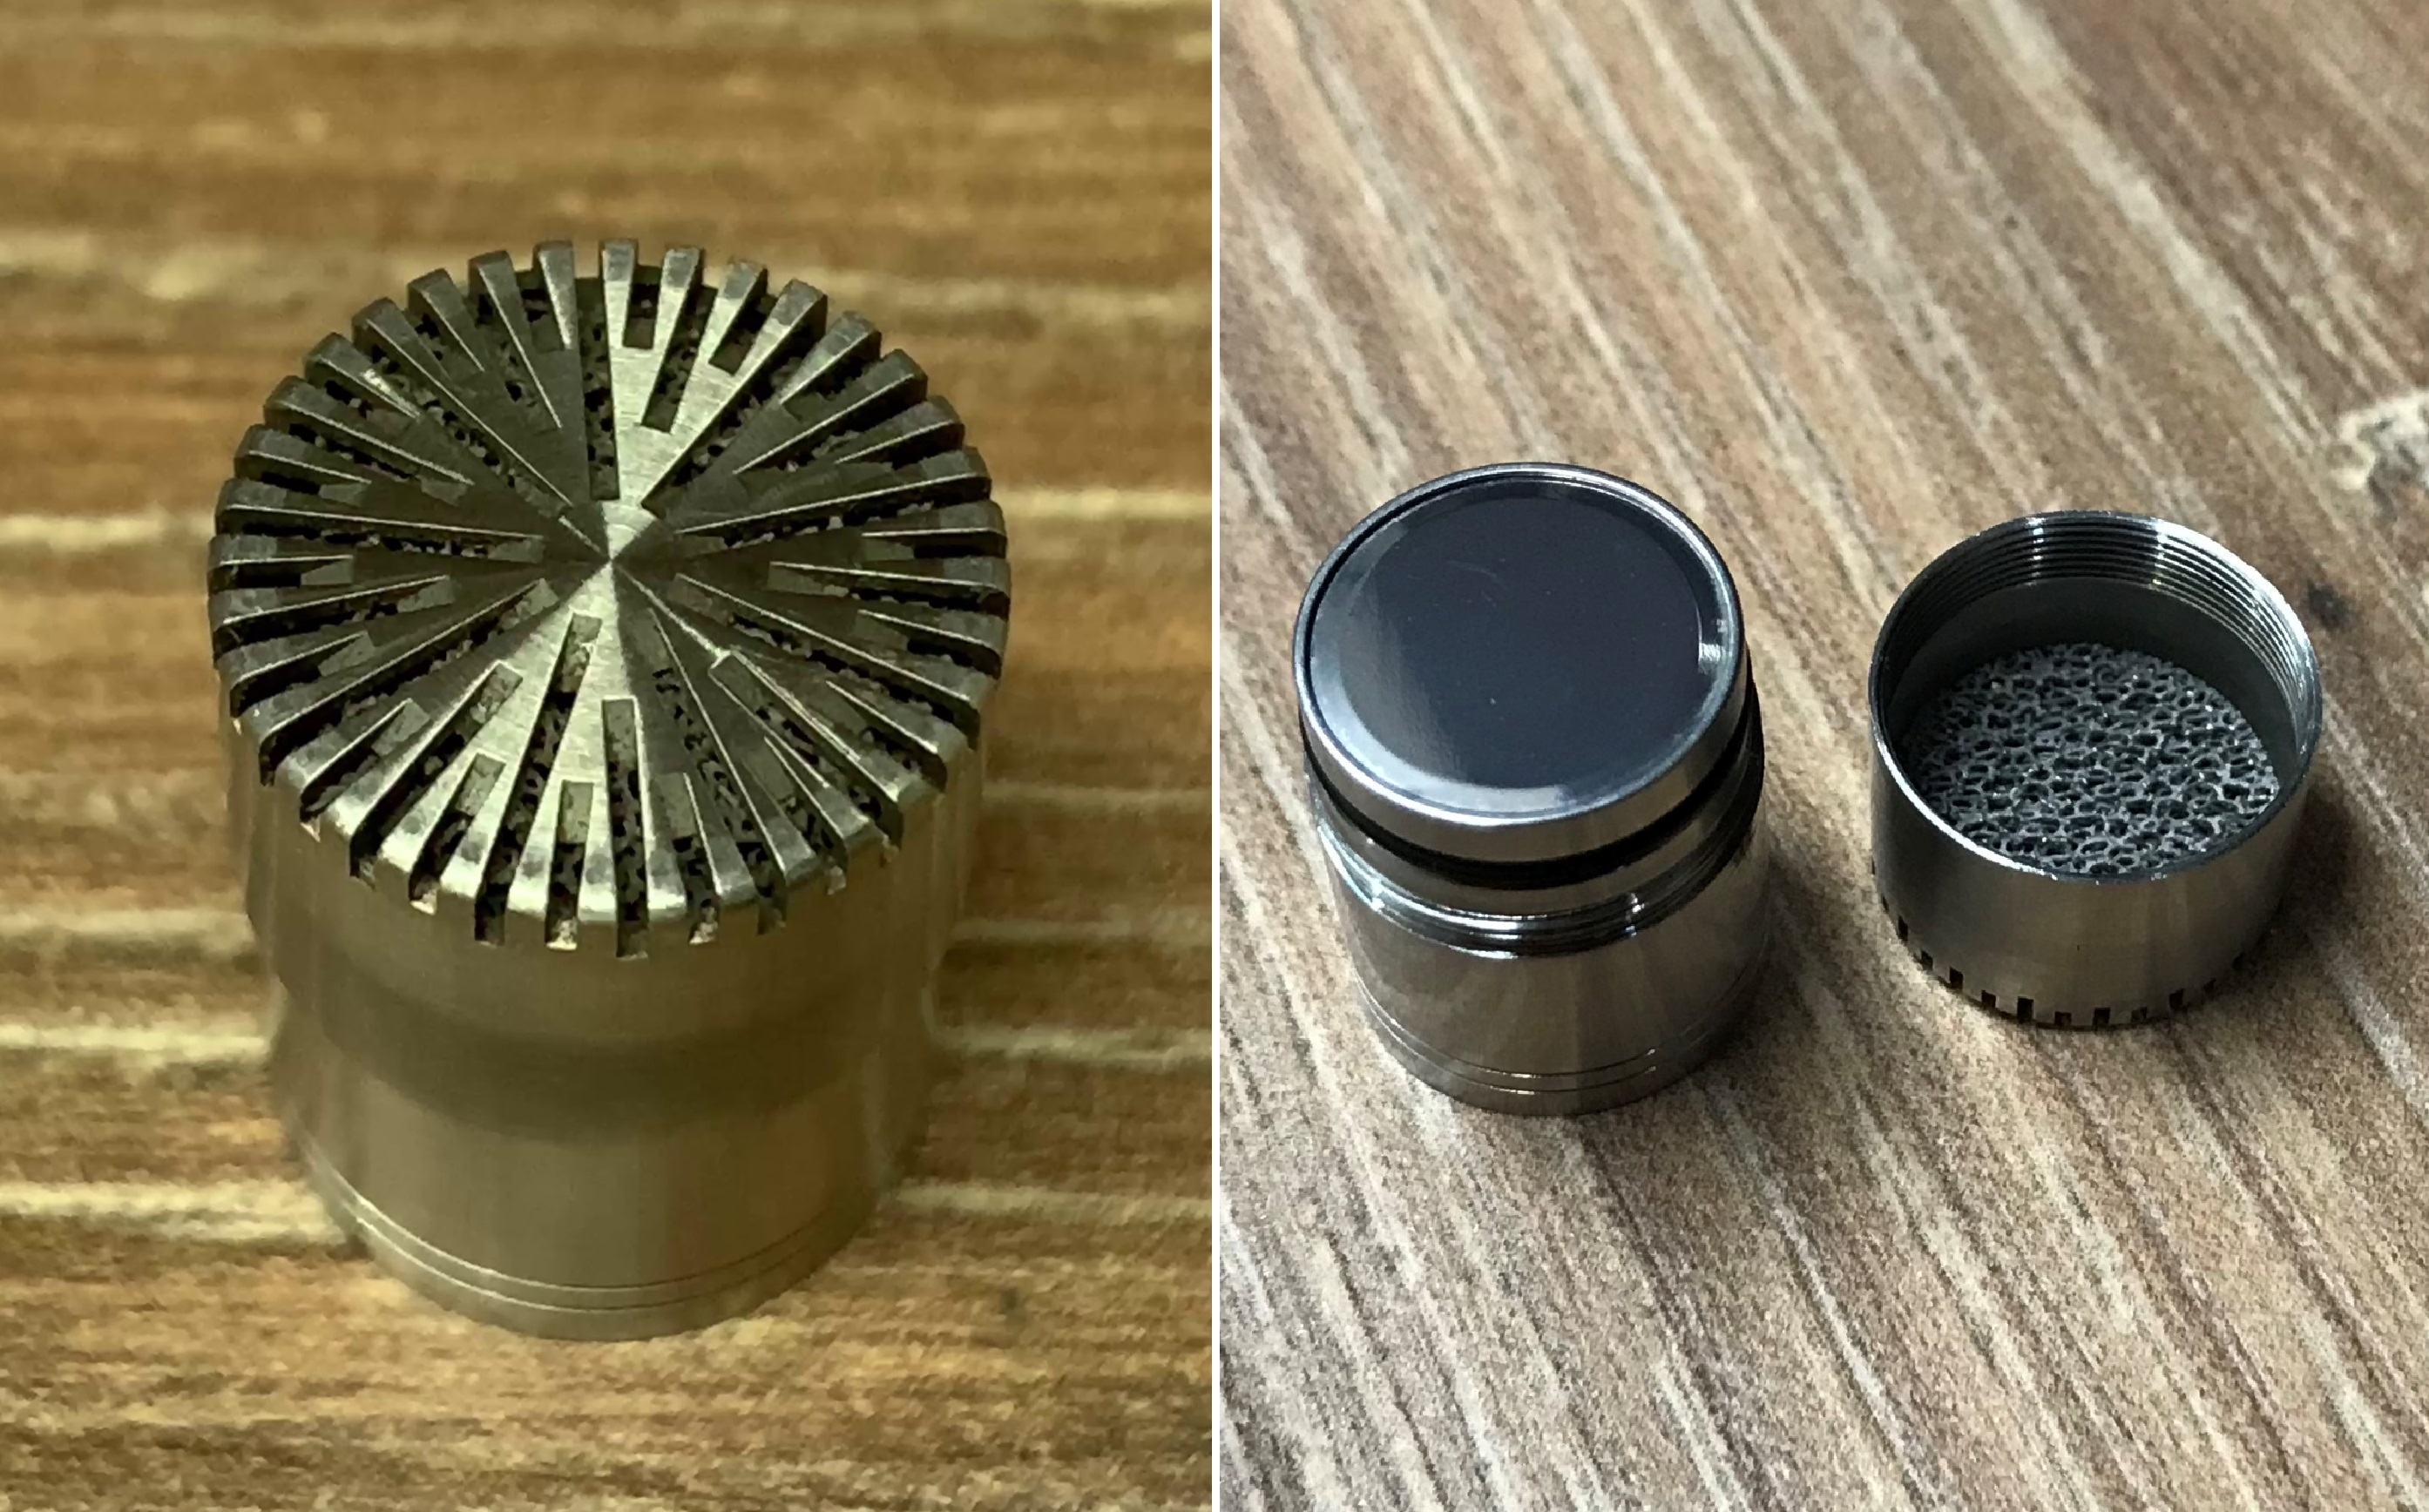
\includegraphics[height=4cm]{2_Metodología/Figs/gras40CE}
        \caption{Micrófono patrón de trabajo GRAS 40CE.}
        \label{fig:gras_40CE}
    \end{subfigure}
\end{figure}
%
\begin{figure}[!h]
    \caption{Instrumentos para adecuación de la señal eléctrica.}
    \centering
    \begin{subfigure}[t]{0.6\textwidth}
        \centering
        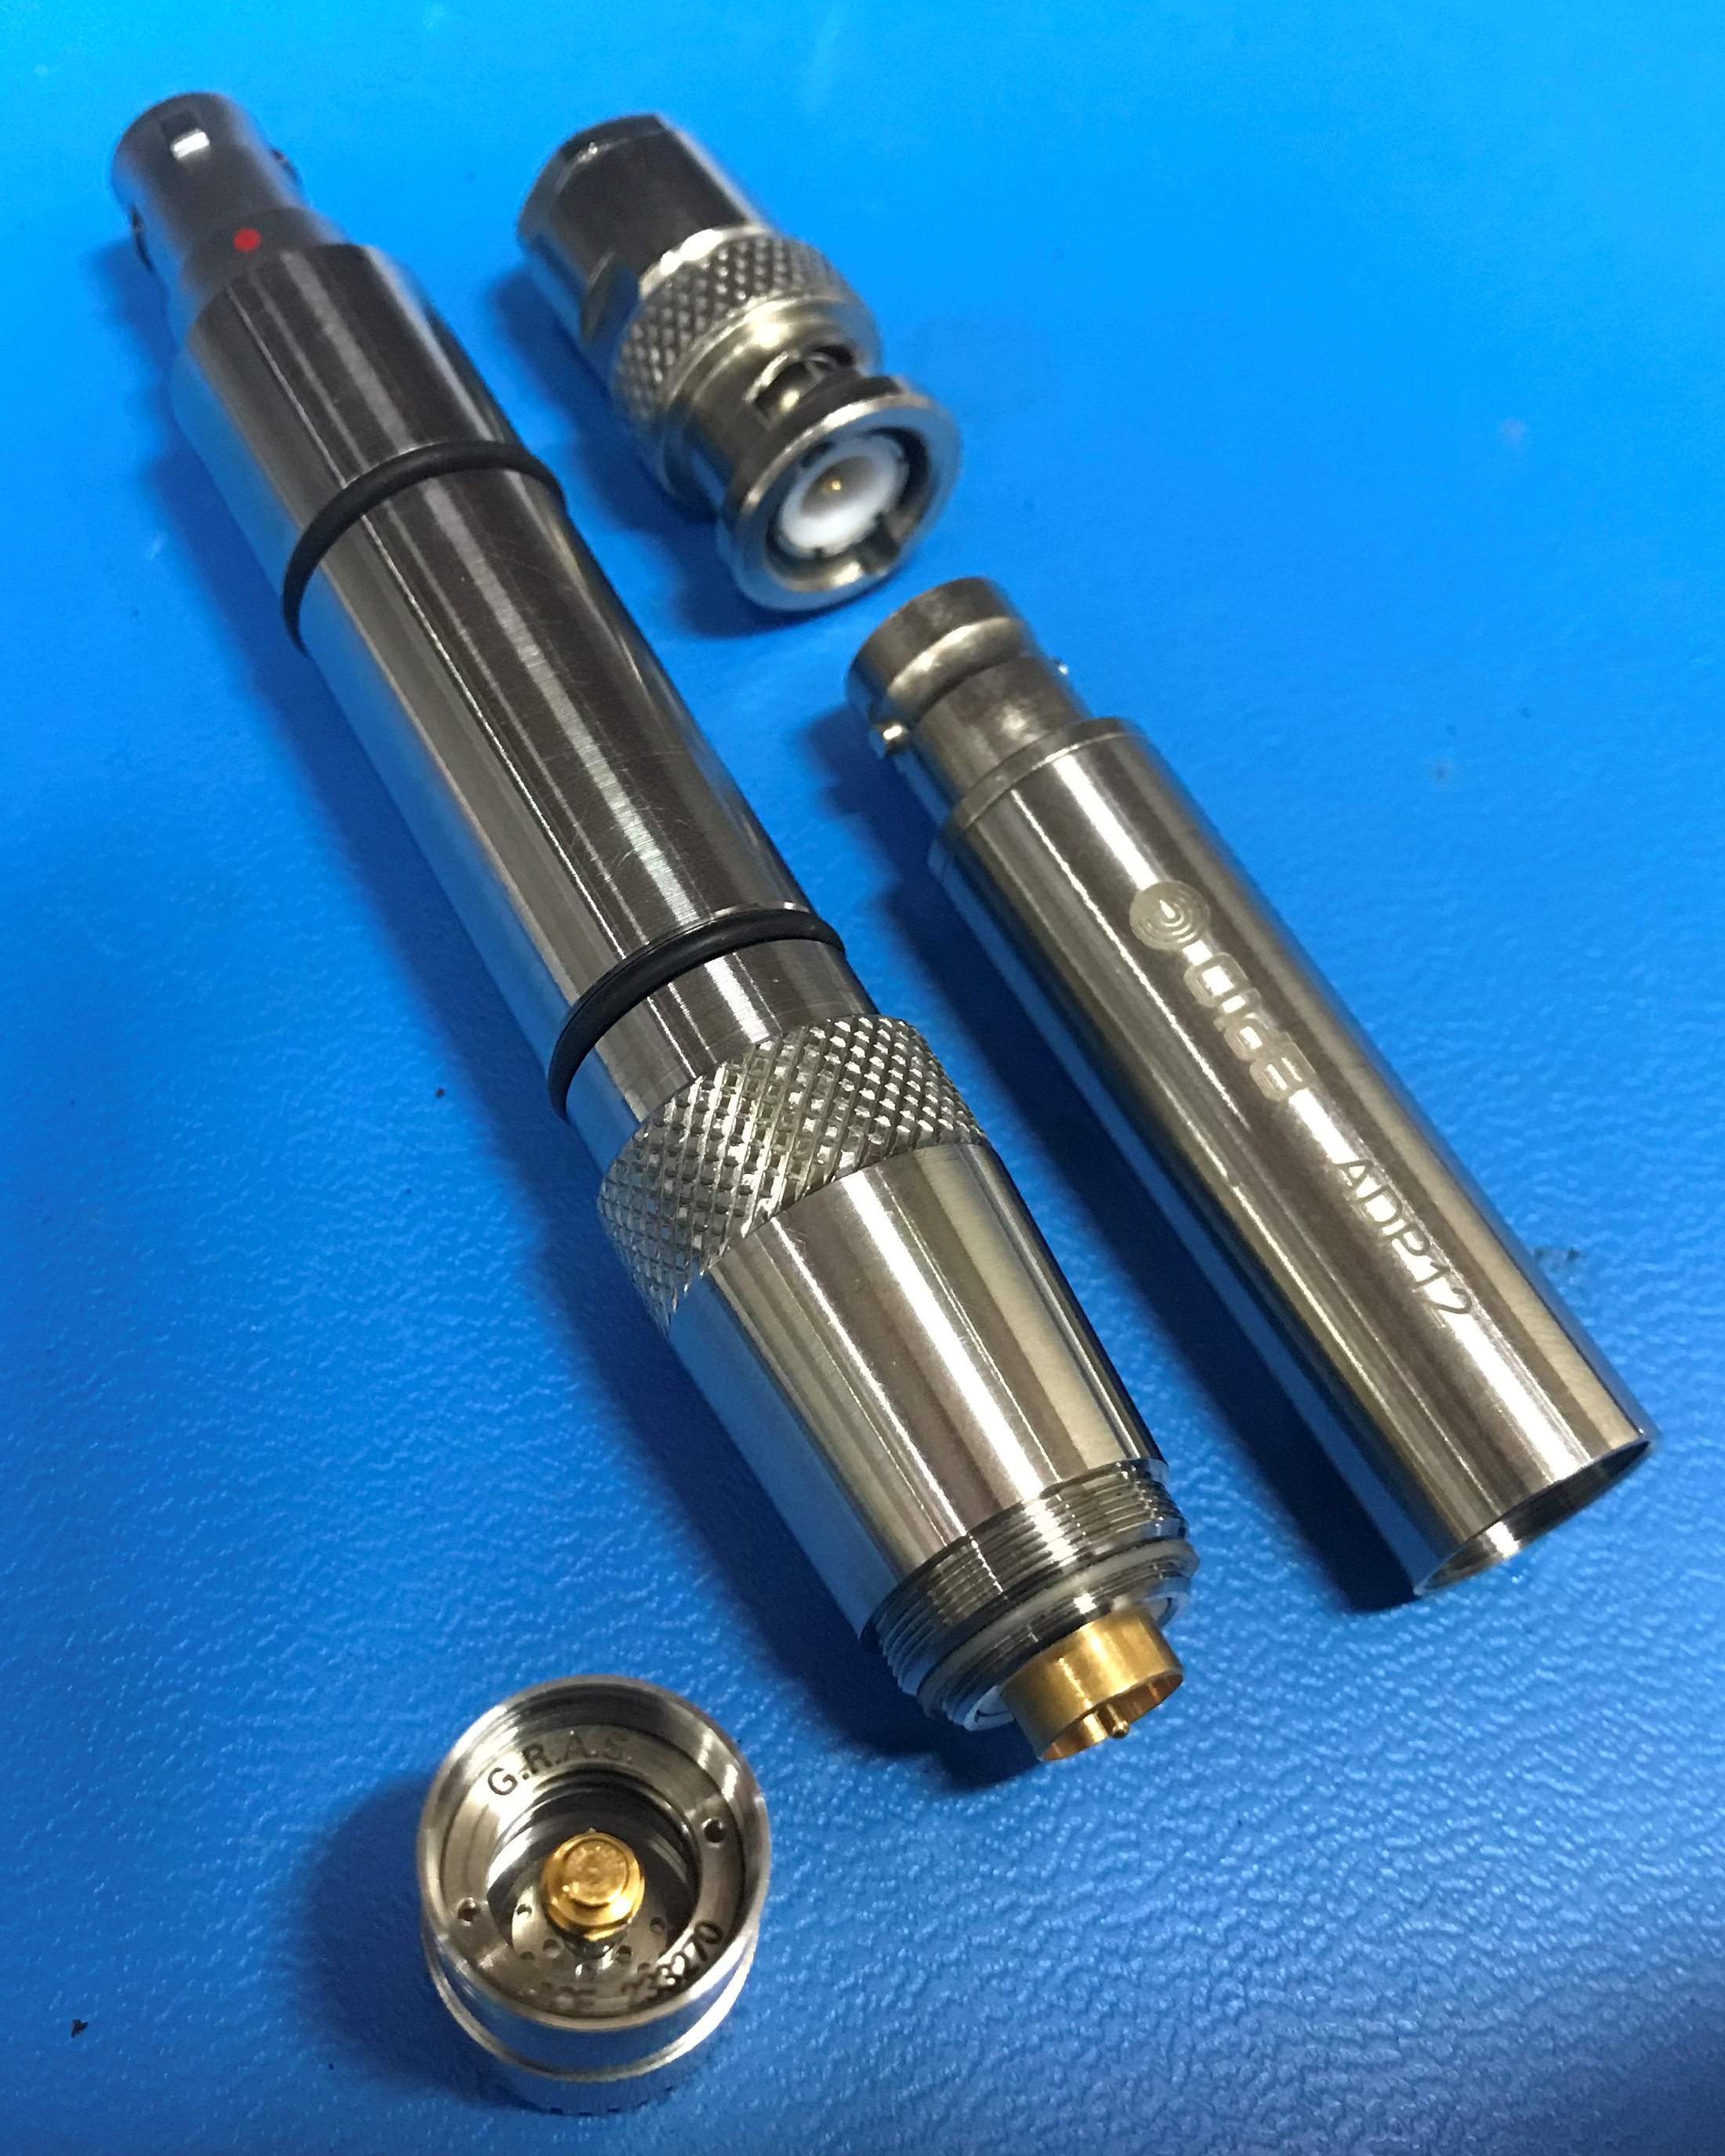
\includegraphics[height=7cm]{2_Metodología/Figs/PRE2201dB}
        \caption{Vista inferior del micrófono GRAS 40CE (izquierda abajo),
            preamplificador para micrófonos de $\nicefrac{1}{2}''$ 01dB PRE22 (medio)
            y adaptador de impedancia 01dB ADP12 con su terminal de aterrizaje (derecha).}
        \label{fig:PRE22_01dB}
    \end{subfigure}
    \hfill
    \begin{subfigure}[t]{0.38\textwidth}
        \centering
        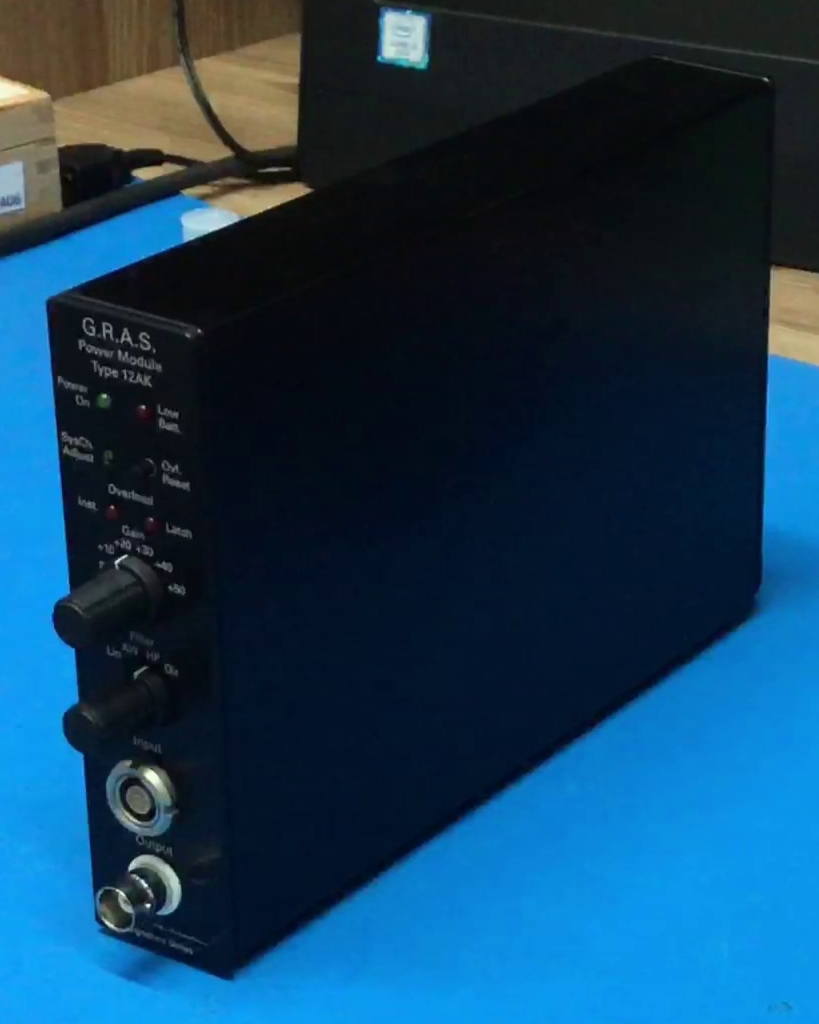
\includegraphics[height=7cm]{2_Metodología/Figs/gras12AK}
        \caption{Módulo de poder para preamplificadores y micrófonos GRAS 12AK.}
        \label{fig:gras_12AK}
    \end{subfigure}
\end{figure}

Como bien indica la norma \mbox{IEC 60942}~\citeyearpar{IEC_TC29_2017}, uno de los posibles métodos para calibrar calibradores acústicos es por comparación contra un calibrador patrón.\ Ese es el método elegido en este trabajo.
El calibrador acústico patrón elegido debe ser de las especificaciones más altas posibles, y su elección también determina el alcance de calibración del laboratorio.
Para este trabajo se emplea el calibrador Brüel \& Kjær 4231 (ver figura~\ref{fig:bruel_4231}), el cual es de clase LS y tiene disponibles dos niveles de presión sonora ($\qtylist{94;114}{\dB}$) a $\qty{1}{\kHz}$.
La trazabilidad de este calibrador se mantiene directamente con el fabricante.

El método requiere también un micrófono de referencia con el cuál se pueda transformar la señal acústica en una señal eléctrica para que pueda ser analizada posteriormente en amplitud, frecuencia y distorsión armónica más ruido (THD+N).
Se empleó el micrófono GRAS 40CE (ver figura~\ref{fig:gras_40CE}), el cual es un micrófono de campo libre con una sensibilidad típica de $\num{40}\,\nicefrac{\unit{\mV}}{\unit{\Pa}}$ y cuenta con su certificado de calibración de fábrica, en el que es posible determinar la diferencia entre las respuestas de campo libre y de campo de presión a $\qty{1}{\kHz}$.

La señal eléctrica del micrófono debe ser adecuada antes de medirla, por lo que se usa un preamplificador 01dB PRE22 (ver figura~\ref{fig:PRE22_01dB}).
Para polarizar el preamplificador se usa un módulo de poder GRAS 12AK, el cual también puede darle mayor ganancia a la señal para mejorar la relación señal a ruido, aplicarle un filtro paso alto para eliminar la interferencia de baja frecuencia y permite hacer el acople de impedancias apropiado para conectar la señal a la entrada de los instrumentos de medición.
Este módulo se muestra en la figura~\ref{fig:gras_12AK}.

\begin{figure}[!h]
    \caption{Instrumentos de medición para la calibración periódica de calibradores acústicos.}
    \centering
    \begin{subfigure}[t]{0.45\textwidth}
        \centering
        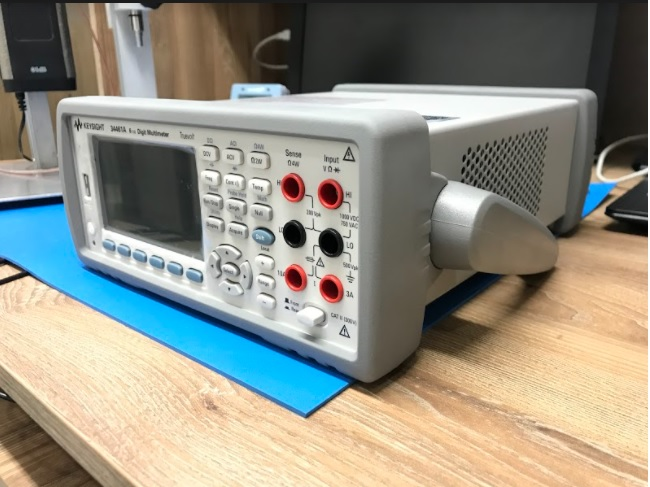
\includegraphics[height=6cm]{2_Metodología/Figs/keysight34461A}
        \caption{Multímetro digital Keysight 34461A.}
        \label{fig:keysight_34461A}
    \end{subfigure}
    \hfill
    \begin{subfigure}[t]{0.45\textwidth}
        \centering
        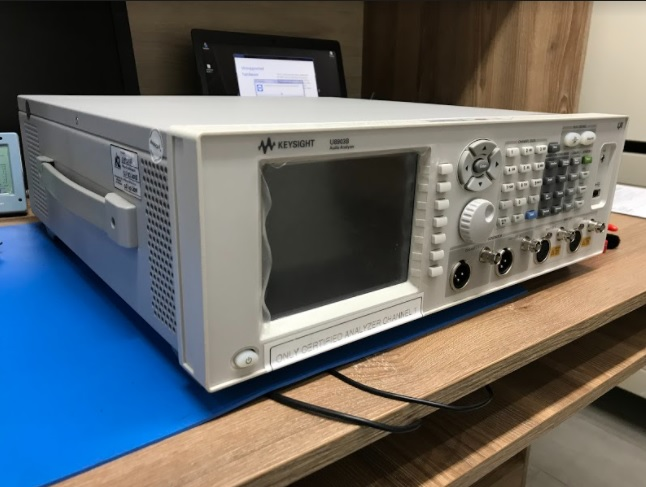
\includegraphics[height=6cm]{2_Metodología/Figs/keysightU8903B}
        \caption{Analizador de audio Keysight U8903B.}
        \label{fig:keysight_U8903B}
    \end{subfigure}
\end{figure}
%
Para medir el voltaje AC y la frecuencia se requiere un multímetro digital con suficientes dígitos de resolución que aporten la precisión requerida y no afecte negativamente la incertidumbre de medición.
El multímetro empleado es el Keysight 34461A de $6\nicefrac{1}{2}$ dígitos (mostrado en la figura~\ref{fig:keysight_34461A}), que, aunque su impacto es proporcional con la escala de medición, en $\unit{\dB}$ resulta ser despreciable.
En $\unit{\Hz}$, debido a la escala lineal, tendrá un impacto mayor, pero sigue siendo despreciable.
Cabe resaltar que, dependiendo de la escala, no todos los dígitos están disponibles en la pantalla del multímetro, pero sí pueden adquirirse todos siempre por la interfaz remota.
Este multímetro mantiene su trazabilidad a los patrones nacionales.

En cuanto a la THD+N, podría usarse una interfaz de sonido con un software de análisis en frecuencia, pero establecer su trazabilidad metrológica es poco factible.
Se requiere un instrumento que igualmente pueda ser calibrado por un laboratorio acreditado para esta magnitud inusual.
Tal es el analizador de audio Keysight U8903B, que cuenta con una resolución de $7$ dígitos, disponibles completamente sólo mediante la interfaz remota.
Este instrumento cuenta con bastantes prestaciones especializadas para el análisis de audio.
Entre estas, unas importantes para los propósitos de este trabajo son: Establecer la impedancia de entrada, tipo de entrada (balanceada o no balanceada), desacople DC de la señal de entrada, filtros paso alto o paso bajo para la entrada, frecuencia de muestreo variable y cálculo de estadísticas en tiempo real.
Este analizador se muestra en la figura~\ref{fig:keysight_U8903B}.

Ambos instrumentos de Keysight cuentan con la interfaz de comunicación GPIB, mediante la cual estos pueden conectarse a un sólo puerto USB del computador para su control con instrucciones SCPI\@.

\subsection{Patrones e instrumentos para la calibración periódica de sonómetros}

\begin{figure}[!h]
    \caption{Esquema de conexiones de los instrumentos para la calibración periódica de sonómetros.}
    \label{fig:IEC61672_connections}
    \begin{subfigure}[t]{0.59\textwidth}
        \centering
        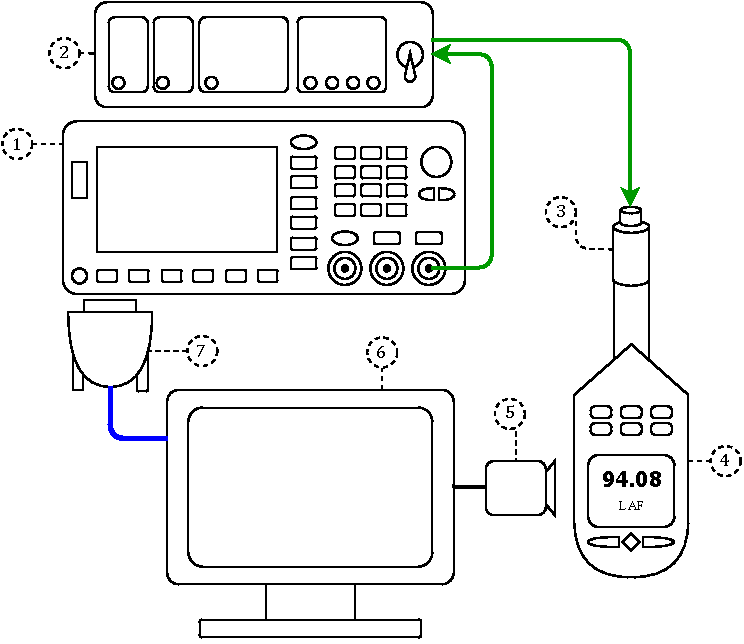
\includegraphics[width=0.95\textwidth]{2_Metodología/Figs/IEC61672-3connections}
    \end{subfigure}
    \hfill
    \begin{subfigure}[t]{0.4\textwidth}
        \centering
        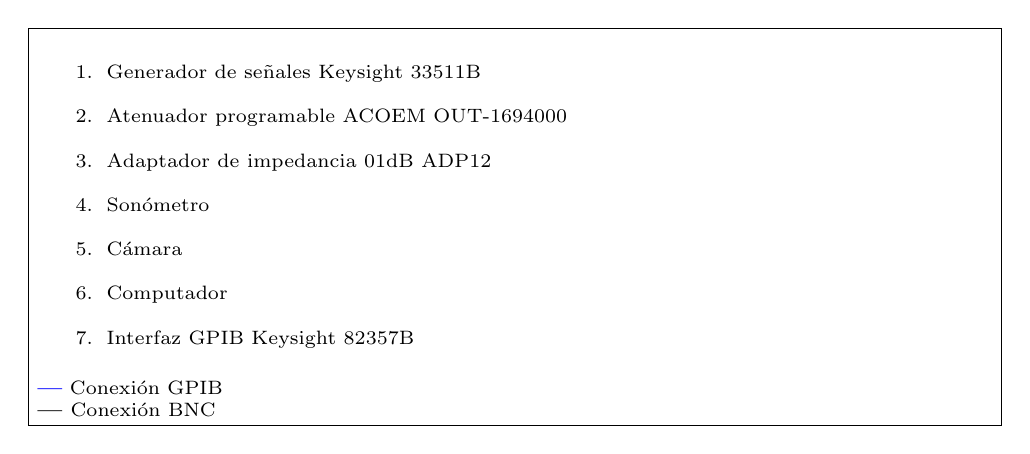
\begin{tikzpicture}
            \node [draw]{\vbox{\scriptsize{
                \begin{enumerate}
                    \item Generador de señales Keysight 33511B
                    \item Atenuador programable ACOEM OUT-1694000
                    \item Adaptador de impedancia 01dB ADP12
                    \item Sonómetro
                    \item Cámara
                    \item Computador
                    \item Interfaz GPIB Keysight 82357B
                \end{enumerate}}
            \textbf{\color{blue} —} Conexión GPIB \\
            \textbf{—} Conexión BNC}};
        \end{tikzpicture}
    \end{subfigure}
    \caption*{\footnotesize Fuente: Elaboración propia.}
\end{figure}

La interconexión propuesta para la calibración de sonómetros se presenta en la figura~\ref{fig:IEC61672_connections}.
A continuación se describe cada instrumento.
%
\clearpage

\begin{figure}[!h]
    \caption{Instrumentos utilizados en la calibración periódica de sonómetros.}
    \centering
    \begin{subfigure}[t]{0.49\textwidth}
        \centering
        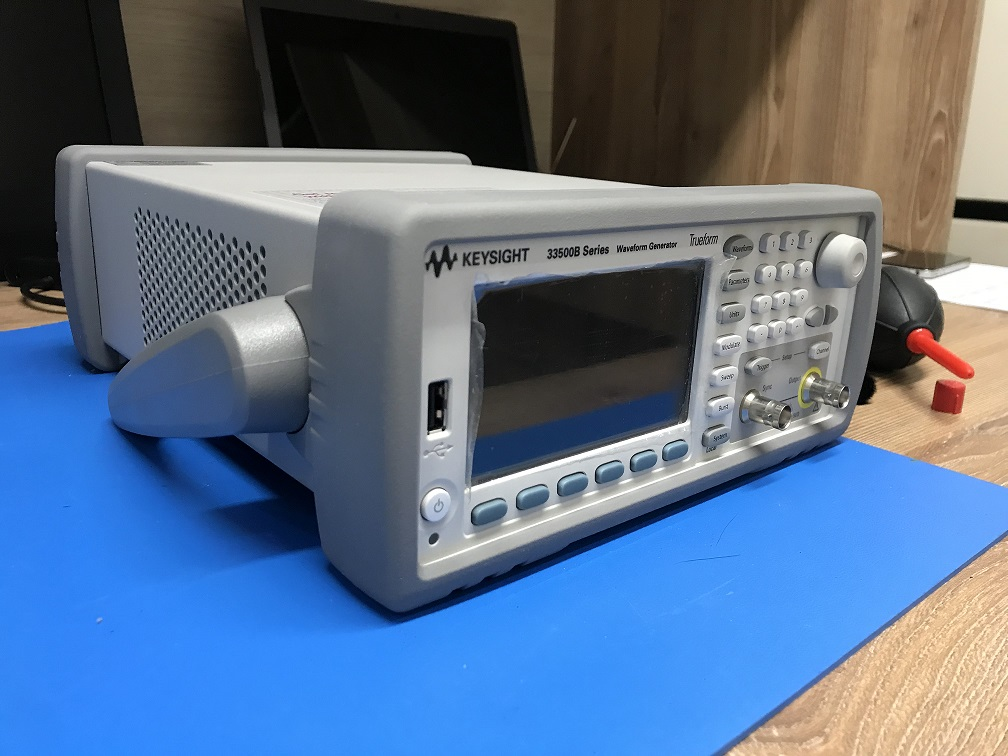
\includegraphics[height=6cm]{2_Metodología/Figs/keysight33511B}
        \caption{Generador de funciones arbitrarias Keysight 33511B.}
        \label{fig:keysight_33511B}
    \end{subfigure}
    \hfill
    \begin{subfigure}[t]{0.49\textwidth}
        \centering
        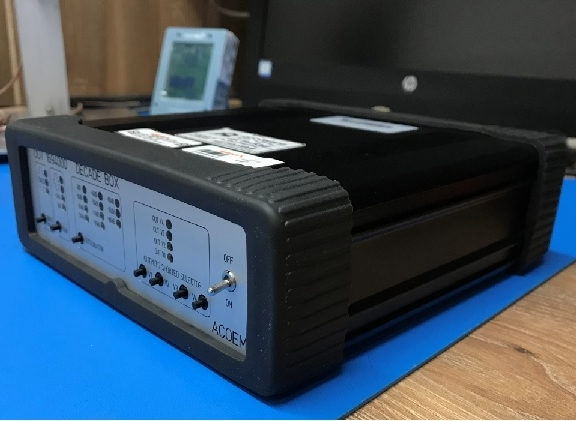
\includegraphics[height=6cm]{2_Metodología/Figs/decadebox}
        \caption{Atenuador programable ACOEM OUT-1694000.}
        \label{fig:decade_box}
    \end{subfigure}
\end{figure}
%
El flujo de señal inicia en el generador de señales.
En este trabajo se empleó el generador de funciones arbitrarias Keysight 33511B (véase figura~\ref{fig:keysight_33511B}), que tiene excelentes prestaciones como la definición personalizada de formas de onda y un desempeño superior dada su baja distorsión armónica (típicamente $\num{0.04}\%$), amplio ancho de banda e intervalo de voltaje, bajo efecto de \emph{jitter}, su filtro \emph{anti-alias}, su resolución de amplitud de $\qty{16}{\bit}$ y de frecuencia de $\qty{1}{\micro\Hz}$, respuesta en frecuencia plana ($\pm\qty{0.10}{\dB}$ en todo el rango inferior a $\qty{100}{\kHz}$), alta precisión en amplitud ($\pm1\%$ del valor establecido $\pm\qty{1}{\mV}$) y en frecuencia ($\pm\qty{2}{ppm}$ del valor establecido $\pm\qty{15}{\pico\Hz}$).
El generador 33511B también cuenta con la interfaz de comunicación GPIB para su control remoto.
Este generador cumple la función de patrón de medición, generando señales eléctricas para \emph{simular} los niveles de presión sonora, y mantiene su trazabilidad a los patrones nacionales.

A pesar de que el generador tiene un rango de voltaje AC amplio ($\qty{1}{\mVpp}$ a $\qty{10}{\Vpp}$), para la mayoría de aplicaciones en sonómetros (cuyos micrófonos tienen sensibilidades típicas entre $\qtyrange{40}{50}{\mV}$), con el fin de alcanzar los niveles más altos (cercanos a los $\qty{140}{\dB}$), se requieren voltajes del orden de $\qty{13}{\Vrms}$ aproximadamente, y para los niveles más bajos (cercanos a los $\qty{23}{\dB}$), se requieren voltajes del orden de $\qty{7}{\uVrms}$.
Por tal motivo se hace necesario un dispositivo adicional que amplifique la señal hasta al menos $\qty{6}{\dB}$ más y que sea capaz de atenuarla hasta al menos $\qty{50}{\dB}$.
Para esto se usó un \emph{Decade Box} o atenuador programable fabricado por ACOEM, el cual se muestra en la figura~\ref{fig:decade_box}.

Finalmente, el flujo de señal termina en el adaptador de impedancias.
Este debe ser preferiblemente el recomendado en el manual de instrucciones del sonómetro, o en su defecto debe usarse uno cuya capacitancia se equipare a la capacitancia del micrófono del sonómetro y que por supuesto tenga el mismo diámetro y rosca.
Como ejemplo, para sonómetros marca 01dB, se utiliza el adaptador 01dB ADP12, que se muestra en la figura~\ref{fig:PRE22_01dB}.

Adicionalmente, para capturar el valor de medición indicado en la pantalla del sonómetro, se usa una cámara web conectada al computador.

\subsection{Comandos SCPI}
\label{subsec:scpi_commands}
En esta sección se explica de forma general el protocolo de comandos estándar para instrumentos programables (SCPI), tomando como guía de referencia el manual del generador Keysight 33511B~\citeyearpar{Keysight2015}.

Los comandos SCPI son un lenguaje basado en ASCII para instrumentos de medición y de pruebas.
Estos comandos están basados en una estructura jerárquica conocida como sistema de árbol, en el que los comandos asociados están agrupados bajo un nodo o raíz común, formando así los subsistemas.
Por ejemplo, una parte de la estructura del sistema \texttt{\small OUTPut} es la siguiente:
%
\begin{Verbatim}[fontsize=\footnotesize]
OUTPut:
    SYNC {OFF|0|ON|1}
    SYNC:
        MODE {NORMal|CARRier}
        POLarity {NORMal|INVerted}
\end{Verbatim}

Las líneas sin sangría son los sistemas raíces y cada nivel de sangría corresponde al nivel del subsistema en la jerarquía.
El ``\textbf{:}" separa una palabra clave de otra en un nivel más bajo.
Las letras en mayúsculas son abreviaciones de las palabras clave de los comandos, que también pueden ser usadas opcionalmente, quitando las letras en minúsculas de la palabra clave.
Las llaves (\textbf{\{\}}), en realidad indican que se esperan los parámetros para un comando dado, los cuales pueden tomar valores numéricos, booleanos, cadenas de texto o palabras clave que denotan valores preestablecidos.
Si un comando espera más de un parámetro, estos son separados por comas.
Por ejemplo, para habilitar la salida del generador ajustándolo en una forma de onda senoidal de $\qty{1}{\kHz}$, con una amplitud de $\qty{50}{\mV}$ y un \emph{offset} DC de $\qty{0}{\V}$, se enviaría el siguiente comando: \texttt{\small APPL:SIN 1E3,50E-3,0.0}.

También se puede reducir la extensión de los códigos usando ``\textbf{;}" para separar instrucciones de un mismo sistema de mayor nivel.
Por ejemplo, la instrucción \texttt{\small TRIG:SOUR BUS; COUNT 30} logra el mismo efecto que las instrucciones \texttt{\small TRIG:SOUR BUS} y \texttt{\small TRIG:COUNT 30} enviadas una tras otra.

Se puede consultar el valor actual de la mayoría de parámetros de sistemas o subsistemas usando ``\textbf{?}". Por ejemplo, con el comando \texttt{\small :CALC:STAT:DATA1?} se obtiene el primer valor estadístico calculado por el analizador de audio, según se haya configurado previamente.

Cada instrumento de Keysight usado en este trabajo cuenta con un conjunto específico de sistemas y subsistemas para realizar las funciones particulares según su naturaleza, los cuales pueden ser consultados en las guías de referencia de comandos SCPI de los respectivos manuales o, de una forma mucho más interactiva, en la aplicación \emph{Command Expert} de Keysight.
También hay comandos comunes a la mayoría de instrumentos como los siguientes: \texttt{\small *IDN?} (consulta la información de identificación del instrumento) y \texttt{\small *TST?} (ejecuta la secuencia de autoverificación del instrumento).

El control remoto de los instrumentos con comandos SCPI se implementó en Python con la librería \texttt{\small PyVisa}~\citeyearpar{PyVisa2022}, la cual requiere que en el computador esté instalada por lo menos la librería VISA de \emph{National Instruments} o, como en este desarrollo, la \emph{Keysight IO Library Suite} \citepalias{Keysight2022}, las cuales son totalmente gratuitas.
